\documentclass[11pt, onesided]{book}

%%%%%%%%%%%%%%Include Packages%%%%%%%%%%%%%%%%%%%%%%%%%%
\usepackage{xcolor}
\usepackage{mathtools}
\usepackage[a4paper, total={6in, 8in}, margin=1.25in]{geometry}
\usepackage{amsmath}
\usepackage{amssymb}
\usepackage{paralist}
\usepackage{rsfso}
\usepackage{amsthm}
\usepackage{wasysym}
\usepackage[inline]{enumitem}   
\usepackage{hyperref}
\usepackage{tocloft}
\usepackage{wrapfig}
\usepackage{titlesec}
\usepackage{colortbl}
\usepackage{stackengine} 
%%%%%%%%%%%%%%%%%%%%%%%%%%%%%%%%%%%%%%%%%%%%%%%%%%%%%%%%


%%%%%%%%%%%%%%%Chapter Setting%%%%%%%%%%%%%%%%%%%%%%%%%%
\definecolor{gray75}{gray}{0.75}
\newcommand{\hsp}{\hspace{20pt}}
\titleformat{\chapter}[hang]{\Huge\bfseries}{\thechapter\hsp\textcolor{gray75}{$\mid$}\hsp}{0pt}{\Huge\bfseries}
%%%%%%%%%%%%%%%%%%%%%%%%%%%%%%%%%%%%%%%%%%%%%%%%%%%%%%%%

%%%%%%%%%%%%%%%%%Theorem environments%%%%%%%%%%%%%%%%%%%
\newtheoremstyle{break}
  {\topsep}{\topsep}%
  {\itshape}{}%
  {\bfseries}{}%
  {\newline}{}%
\theoremstyle{break}
\theoremstyle{break}
\newtheorem{axiom}{Axiom}
\newtheorem{thm}{Theorem}[section]
\renewcommand{\thethm}{\arabic{section}.\arabic{thm}}
\newtheorem{lem}{Lemma}[thm]
\newtheorem{cor}{Corollary}[thm]
\newtheorem{defn}{Definition}[thm]
\newenvironment{indEnv}[1][Proof]
  {\proof[#1]\leftskip=1cm\rightskip=1cm}
  {\endproof}
%%%%%%%%%%%%%%%%%%%%%%%%%%%%%%%%%%%%%%%%%%%%%%%%%%%%%%


%%%%%%%%%%%%%%%%%%%%%%%Integral%%%%%%%%%%%%%%%%%%%%%%%
\def\upint{\mathchoice%
    {\mkern13mu\overline{\vphantom{\intop}\mkern7mu}\mkern-20mu}%
    {\mkern7mu\overline{\vphantom{\intop}\mkern7mu}\mkern-14mu}%
    {\mkern7mu\overline{\vphantom{\intop}\mkern7mu}\mkern-14mu}%
    {\mkern7mu\overline{\vphantom{\intop}\mkern7mu}\mkern-14mu}%
  \int}
\def\lowint{\mkern3mu\underline{\vphantom{\intop}\mkern7mu}\mkern-10mu\int}
%%%%%%%%%%%%%%%%%%%%%%%%%%%%%%%%%%%%%%%%%%%%%%%%%%%%%%



\newcommand{\R}{\mathbb{R}}
\newcommand{\N}{\mathbb{N}}
\newcommand{\Z}{\mathbb{Z}}
\newcommand{\Q}{\mathbb{Q}}
\newcommand{\C}{\mathbb{C}}
\newcommand{\T}{\mathcal{T}}
\newcommand{\M}{\mathcal{M}}
\newcommand{\Symm}{\text{Symm}}
\newcommand{\Alt}{\text{Alt}}
\newcommand{\Int}{\text{Int}}
\newcommand{\Bd}{\text{Bd}}
\newcommand{\Power}{\mathcal{P}}
\newcommand{\ee}[1]{\cdot 10^{#1}}
\newcommand{\spa}{\text{span}}
\newcommand{\sgn}{\text{sgn}}
\newcommand{\degr}{\text{deg}}
\newcommand{\pd}{\partial}
\newcommand{\that}[1]{\widetilde{#1}}
\newcommand{\lr}[1]{\left(#1\right)}
\newcommand{\vmat}[1]{\begin{vmatrix} #1 \end{vmatrix}}
\newcommand{\bmat}[1]{\begin{bmatrix} #1 \end{bmatrix}}
\newcommand{\pmat}[1]{\begin{pmatrix} #1 \end{pmatrix}}
\newcommand{\rref}{\xrightarrow{\text{row\ reduce}}}
\newcommand{\txtarrow}[1]{\xrightarrow{\text{#1}}}
\newcommand\oast{\stackMath\mathbin{\stackinset{c}{0ex}{c}{0ex}{\ast}{\Circle}}}
\newcommand{\txt}{Wald's \textit{General Relativity}}

\newcommand{\note}{\color{red}Note: \color{black}}
\newcommand{\remark}{\color{blue}Remark: \color{black}}
\newcommand{\example}{\color{green}Example: \color{black}}
\newcommand{\exercise}{\color{green}Exercise: \color{black}}

%%%%%%%%%%%%%%%%%%%%%%Roman Number%%%%%%%%%%%%%%%%%%%%%%%
\makeatletter
\newcommand*{\rom}[1]{\expandafter\@slowromancap\romannumeral #1@}
\makeatother
%%%%%%%%%%%%%%%%%%%%%%%%%%%%%%%%%%%%%%%%%%%%%%%%%%%%%%%%%

%%%%%%%%%%%%%table of contents%%%%%%%%%%%%%%%%%%%%%%%%%%%%
%\setlength{\cftchapindent}{0em}
%\cftsetindents{section}{2em}{3em}
%
%\renewcommand\cfttoctitlefont{\hfill\huge\bfseries}
%\renewcommand\cftaftertoctitle{\hfill\mbox{}}
%
%\setcounter{tocdepth}{2}
%%%%%%%%%%%%%%%%%%%%%%%%%%%%%%%%%%%%%%%%%%%%%%%%%%%%%%%%%%


%%%%%%%%%%%%%%%%%%%%%Footnotes%%%%%%%%%%%%%%%%%%%%%%%%%%%
\newcommand\blfootnote[1]{%
  \begingroup
  \renewcommand\thefootnote{}\footnote{#1}%
  \addtocounter{footnote}{-1}%
  \endgroup
}
%%%%%%%%%%%%%%%%%%%%%%%%%%%%%%%%%%%%%%%%%%%%%%%%%%%%%%%%%

%%%%%%%%%%%%%%%%%%%%%Section%%%%%%%%%%%%%%%%%%%%%%%%%%%%%
\makeatletter
\def\@seccntformat#1{%
  \expandafter\ifx\csname c@#1\endcsname\c@section\else
  \csname the#1\endcsname\quad
  \fi}
\makeatother
%%%%%%%%%%%%%%%%%%%%%%%%%%%%%%%%%%%%%%%%%%%%%%%%%%%%%%%%%

%%%%%%%%%%%%%%%%%%%%%%%%%%%%%%%%%%%Enumerate%%%%%%%%%%%%%%
\makeatletter
% This command ignores the optional argument 
% for itemize and enumerate lists
\newcommand{\inlineitem}[1][]{%
\ifnum\enit@type=\tw@
    {\descriptionlabel{#1}}
  \hspace{\labelsep}%
\else
  \ifnum\enit@type=\z@
       \refstepcounter{\@listctr}\fi
    \quad\@itemlabel\hspace{\labelsep}%
\fi}
\makeatother
\parindent=0pt
%%%%%%%%%%%%%%%%%%%%%%%%%%%%%%%%%%%%%%%%%%%%%%%%%%%%%%%%%%



\begin{document}

	\begin{titlepage}
		\begin{center}
			\vspace*{0.5cm}
			\Huge \color{red}
				\textbf{Class Notes}\\
			\vspace{0.5cm}			
			\Large \color{black}
			Physics 535 - General Relativity\\
			Professor Leopoldo A. Pando Zayas
			\vspace{1.5cm}

			
\includegraphics[scale=1.15]{hmm.pdf}
			
			
			\vspace{2cm}
			\LARGE
				\textbf{Jinyan Miao}\\
				\hfill\break
				\LARGE Fall 2023\\
			\vspace{1cm}

		\vspace*{\fill}
		\end{center}			
	\end{titlepage}



\tableofcontents
\hfill\break
\hfill\break
\hfill\break
 

\newpage
\section[Technicalities]{\color{red}Technicalities\color{black}}
\subsection*{Hyperbolic functions}
\begin{align*}
\sinh(x) = \frac{e^x - e^{-x}}{2}\,,\qquad
\cosh(x) = \frac{e^x + e^{-x}}{2}\,,\qquad
\tanh = \frac{\sinh(x)}{\cosh(x)} = \frac{e^x - e^{-x}}{e^x+ e^{-x}}\,.
\end{align*}
\begin{align*}
\frac{d}{dx}\sinh(x) = \cosh(x)\,,\qquad
\frac{d}{dx}\cosh(x) = \sinh(x)\,,\qquad
\frac{d}{dx}\tanh(x) = 1-\tanh^2(x)\,.
\end{align*}
\begin{align*}
\sinh(-x) = -\sinh(x) \,,\qquad \cosh(-x) = \cosh(x) \,,\qquad
\tanh(-x) = -\tanh(x)\,.
\end{align*}
\begin{align*}
\cosh^2(x) - \sinh^2(x) =1\,,\qquad
\text{sech}^2(x) = 1- \tanh^2(x)\,,\qquad
\text{csch}^2(x) = \text{coth}^2(x)-1\,.
\end{align*}
\begin{align*}
\sinh(x+y) &= \sinh(x) \cosh(y) + \cosh(x) \sinh(y)\,,\\
\cosh(x+y) &= \cosh(x) \cosh(y) + \sinh(x) \sinh(y)\,,\\
\tanh(x+y) &= (\tanh(x) + \tanh(y))({1+ \tanh(x) \tanh(y)})^{-1}\,.
\end{align*}
\subsection*{Trigonometric functions}
\begin{align*}
\sin(2\theta) = 2\sin(\theta) \cos(\theta)\,,\qquad
\cos(2\theta) = \cos^2(\theta) - \sin^2(\theta) = 2\cos^2(\theta)-1\,.
\end{align*}
\begin{align*}
e^{iz} = \cos(z) + i\sin(z)\,,\qquad \sin(z) = \frac{e^{-z} - e^{-iz}}{2i}\,,\qquad \cos(z) = \frac{e^{iz} + e^{-iz}}{2}\,.
\end{align*}
\subsection*{Calculus}
Integration by parts,
\begin{align*}
\int_a^b u(x)\,v(x)\, dx = \left[u(x)\int v(x) \, dx\right]_a^b - \int_a^b \left(u'(x)\int v(x)\, dx \right)\,dx
\end{align*}
Leibniz Rule,
\begin{align*}
\frac{d}{dx}\left(\int_{a(x)}^{b(x)}
f(x,t) \, dt
\right) = f(x,b(x)) \cdot \frac{d}{dx}b(x) - f(x,a(x)) \cdot \frac{d}{dx}a(x) + \int_{a(x)}^{b(x)}\frac{\pd}{\pd x}f(x,t)\, dt\,.
\end{align*}
For Lagrangian $\mathcal{L}(\vec{q}(t),\dot{\vec{q}}(t))$, minimizing $S = \int \mathcal{L}(\vec{q}(t),\dot{\vec{q}}(t))\, dt\, $, with $\vec{q}\in \R^n$,
\begin{align*}
\frac{\pd \mathcal{L}}{\pd q^i} - \frac{d}{dt}\frac{\pd \mathcal{L}}{\pd \dot{q}^i} = 0\,,\qquad\qquad\text{for }i\in \N_n\,.
\end{align*}
Taylor expansion of $f(x)$ around $x = a$, 
\begin{align*}
f(x) =\sum_{n=0}^\infty \frac{f^{(n)}(a)}{n!}\, (x-a)^n =f(a) + \frac{f'(a)}{1!}(x-a) + \frac{f''(a)}{2!}(x-a)^2 + \frac{f'''(a)}{3!}(x-a)^3 + \cdots\,.
\end{align*}

\newpage
\chapter{Preliminaries}
\quad Any theory of gravity should be able to answer the problem of how gravitational interaction is characterized in a presence of a mass, and from Newton's point of view, gravitational potential $\phi$ is related to mass density $\rho$ by $\nabla^2 \phi = 4\pi G\rho$, or expressed in the Gauss law,
\begin{align*}
\oint_S \vec{g}\cdot d\vec{s} = 4\pi Gm
\end{align*}
where $m$ is a mass enclosed by the surface $S$ and $\vec{g}$ is the gravitational field. While in General Relativity (GR), Einstein's Field Equation characterizes the gravitation interaction. Furthermore, the theory should also be able to determine the motion of particles that feels the gravity, and from Newton's point of view $-\nabla \phi = a$ gives the acceleration of the particle, while in GR, the motion of particles is characterized by geodesics in spacetime. 

\section[$k$-Calculus]{\color{red}$k$-Calculus\color{black}}
\textit{Here we will develop some geometric intuition for relativity and construct the picture of spacetime diagram.} \\

\subsection{Galileo Transformations}
A point in spacetime is referred as an event, denoted as $(t,\vec{x})$. An observer in spacetime has a \textit{clock} and a \textit{ruler} to measure distance between points in spacetime, while in GR, there is no preferred observers. Hence one would like to study the transformation of observations by different observer in spacetime. From Galileo, one of those transformations can be characterized by the following, perhaps with carefully chosen coordinates, 
\begin{align*}
 x = x' + vt,\qquad y=y', \qquad z = z',\qquad t=t'.
\end{align*}
where $(t,x,y,z)$ and $(t',x',y',z')$ are measurements taken by two different observers. Note here, in Galileo transformations, the force acting on an object is invariant between observers, that is $m\ddot{x} = m\ddot{x}'$. \\

\subsection{Model of Special Relativity}
Now consider the context of special relativity, where we take the speed of light as $c = 1$. We have the two postulate for special relativity: (1) The laws of physics take the same form in every inertial frame. This is also known as the postulate of equivalence of inertial observers. (2) The speed of light, $c$, is the same in all inertial frames.\\

Suppose $A$ sends a light signal to $B$ moving away from $A$ at $t=0$, and after a time $T$, $A$ sends another light signal to $B$. From $B$'s point of view, the time interval between the two signals received by $B$ can be denoted as $kT$ with some $k \in \R$. Meanwhile, $B$ sends signals back to $A$ immediately after receiving the signals from $A$. Then by principle of relativity, from $A$'s point of view, the time interval between the first time $A$ receives a signal from $B$ and the time when $A$ receives the second signal from $B$ is given by $k^2 T$. If $A$ and $B$ are at the same place when $A$ sends the first signal to $B$, then from $A$'s point of view, $A$ can conclude that the coordinate for $B$ when $B$ sends the second signal back to $A$ is given by
\begin{align*}
(t,x) = \left( \frac{k^2T - T}{2} + T, \ \frac{k^2 T-T}{2}\right) = \left( \frac{1}{2}(k^2+1) T, \ \frac{1}{2}(k^2 - 1) T\right)\,,
\end{align*}
and the speed of $B$, in the point of view of $A$, can then be computed as
\begin{align*}
v = \frac{k^2 - 1}{k^2 +1}\,,
\end{align*}
where we see here we have a $k$-factor from $A$'s point of view
\begin{align}
k(v) = \sqrt{\frac{1+v}{1-v}}
\end{align}
characterizes the Doppler Effect, $k>1$ when $B$ is moving from $A$, and $k<1$ when $B$ is approaching $A$. \\


Now consider there are three inertial frames $A,\,B,\,C$. From $A$'s point of view, $B$ is moving with speed $v_{AB}$, with $k$-factor $k_{AB}$. Notice that we have $k_{BC} k_{AB}T = k_{AC}T$. Hence we have $k_{AC} = k_{AB} k_{BC}$, from which one can apply (1.1) to derive 
\begin{align}
v_{AC} = \frac{v_{AB}+v_{BC}}{1+v_{AB}v_{BC}}\,.
\end{align}
Note here for $v_{AB}\ll 1$ and $v_{BC}\ll 1$, we have $v_{AC} = v_{AB} + v_{BC}$. If $v_{BC} = 1$, we then have $v_{AC} =1$. Furthermore, if one object has speed smaller than $1$ in one frame, then its speed is smaller than $1$ in all frames. Note from here also that (1.2) characterizes the Lorentz transformation. \\

Now consider one wants to describe an event $p=(x,t) = (x',t')$ in spacetime in the unprimed $S$ frame and primed $S'$ frame. Observer $A$ in $S$ frame sends out a light signal at time $t - x$ which illuminates $p$ at time $t$, $A$ also receives the reflected light signal from $p$ at time $t+x$. 
\begin{center}
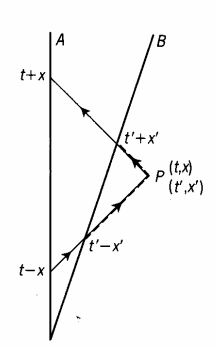
\includegraphics[scale=0.9]{LT.png}
\end{center}
From here we can write
\begin{align*}
t'-x' = k(t-x) \,,\qquad t+x = k(t'+x')\,.
\end{align*}
Rearranging we obtain the Lorentz transformation
\begin{align*}
t' = \frac{t-vx}{\sqrt{1-v^2}}\,,\qquad x' = \frac{x - vt}{\sqrt{1-v^2}}\,,
\end{align*}
from which we see that we have $t'{}^2 - x'{}^2 = t^2 - x^2$. More generally, one can write
\begin{align}
s^2 = (t_1-t_2)^2 - (x_1 - x_2)^2 - (y_1 - y_2)^2 -(z_1-z_2)^2\,,
\end{align}
where $(t_i,x_i,y_i,z_i)$ is the coordinate in the $S_i$ frame, and $S_1$ and $S_2$ frames are related via a Lorentz transformation. A metric that restates (1.3) has the form
\begin{align}
ds^2 = dt^2 - dx^2 - dy^2 - dz^2\,.
\end{align}
A spacetime manifold of dimension $4$ in which the metric (1.4) is invariant is called the Minkowski space. \\

\section[Lorentz Transformation]{\color{red} Lorentz Transformation\color{black}}
In the model of special relativity, it is not hard to observe that, coordinates $(t,x,y,z)$ and $(t',x',y',z')$ in inertial frames $S$ and $S'$ are related via a linear transformation $L$ that is independent on the coordinates,
\begin{align*}
\bmat{t'\\x'\\y'\\z'} = L \bmat{t\\x\\y\\z}\,,
\end{align*}
which is a statement corresponds to the principle of special relativity.\\

On the other hand, the constancy of speed of light ensures that, for the coordinates of a light traveling in frame $S$ or $S'$, we have
\begin{align*}
I = c^2t^2 - x^2 - y^2 - z^2 = c^2t'{}^2 - x'{}^2 - y'{}^2 - z'{}^2 =  I' = 0\,.
\end{align*}
If the two frames are moving relative to each other in the $x$-direction only, with speed $v$, then $y=y'$ and $z=z'$ from which one obtain $-c^2 t^2 + x^2 = -c^2 t'{}^2 + x'{}^2$. Introducing the imaginary time $T = ict$, one can write
\begin{align}
T^2 +x^2 = T'{}^2 + x'{}^2\,.
\end{align}
The family of solution to (1.5) has the form
\begin{align}
x' = x \cos(\theta) + T\sin(\theta)\,,\qquad T'= -x\sin(\theta) + T\cos(\theta)\,,
\end{align}
or in its matrix form
\begin{align}
\bmat{T' \\ x' \\ y' \\ z'} = \bmat{\cos(\theta) & -\sin(\theta) & 0  & 0 \\
\sin(\theta) & \cos(\theta) & 0& 0\\
0 & 0 & 1 & 0\\
0 & 0 & 0 & 1}
\bmat{T \\ x \\ y \\z}\,.
\end{align}
It can be found easily, via the imposition that $x' = 0$, $x = vt+x' = vt$, that (1.6) indicates $\theta$ and $v$ are related by
\begin{align*}
\tan(\theta)  = \frac{iv}{c}\,,
\end{align*}
where $v$ is the relative speed between $S$ and $S'$.\\

Utilizing (1.7), one obtains
\begin{align}
 x' = \beta (x - vt) \,,\qquad t' = \beta (1- vx/c^2)\,,
\end{align}
where $\beta = 1/\sqrt{1 - v^2 / c^2}$. It is not hard to observe from here that the Lorentz transformation has a group structure with the one corresponds to $v = 0$ being the identity. The ones correspond to $v$ and $-v$ are inverse of each other, and composition of any two is also a Lorentz transformation. \\

\subsection{Acceleration in Special Relativity}
Here we consider a particle in motion with velocity $(u_1,u_2,u_3)$ in unprimed frame $S$, and velocity $(u_1', u_2', u_3')$ in primed frame $S'$. From (1.2) we have
\begin{align*}
u_1 = \frac{u_1' + v}{1+ u'_1 v/c^2}
\end{align*}
if the two frames are moving relative to each other via
\begin{align*}
t' = \beta(t-vx/c^2)\,, \qquad x' = \beta (x- vt)\,, \qquad y'=y\,, \qquad z'=z\,,
\end{align*}
where $\beta = 1/\sqrt{1-v^2/c^2}$.\\

The differential of $u_1$ reads
\begin{align*}
du_1 = \frac{1}{\beta^2} \frac{du_1'}{(1+u'_1 v/c^2)^2}\,.
\end{align*}
From (1.8) we have
\begin{align*}
dt = \beta (1 + u_1'v/c^2)\, dt'\,.
\end{align*}
Combining we have
\begin{align*}
\frac{du_1}{dt} = \frac{1}{\beta^3(1+ u'_1 v/c^2)^3}\frac{du_1'}{dt'}\,.
\end{align*}
Similarly we can derive
\begin{align*}
\frac{du_2}{dt} &= \frac{1}{\beta^2(1+u_1v/c^2)^2} \frac{du_2'}{dt'} - \frac{vu_2'}{c^2 \beta^2 ( 1+ u_1'v/c^2)^3}\frac{du_1'}{dt'}\,,\\
\frac{du_3}{dt} &= \frac{1}{\beta^2(1+u_1'v/c^2)^2}\frac{du_3'}{dt'} - \frac{vu_3'}{c^2 \beta^2 (1+ u_1'v/c^2)^3}\frac{du_1'}{dt'}\,.
\end{align*}
Here we see that the acceleration is not an invariant in special relativity, instead, the acceleration is an absolute quantity. That is, if an object is accelerating in one frame, then it is accelerating in all frames; If the object is not accelerating in one frame, then in all frames the object is not accelerating. \\

\subsection{Uniform Acceleration}
The Newtonian definition of a particle moving under uniform acceleration is $du/dt$ being constant, while this cannot hold in special relativity as it implies $u$ approaching infinity as $t$ approaches infinity. Therefore, we here adopt a different definition that acceleration is said to be uniform in special relativity if acceleration is unchanged in any co-moving frame with respect to the moving object. \\

That is, at each instant, the acceleration in an inertial frame traveling with the same velocity as the moving particle has the same value. \\

\example A spaceship whose motor is set at a constant emission rate is uniformly accelerated. Taking the velocity of the particle co-moving with the spaceship to be $u$ in an unprimed frame $S$, then at any instant in a co-moving frame $S'$ has speed $v = u$ moving away from $S$.  In $S'$, the co-moving particle has $u' = 0$, and $du'/dt' = a$ as the constant. From here we can write
\begin{align*}
\frac{du}{dt} = \frac{1}{\beta^3} a\,,
\end{align*}
which has solution 
\begin{align*}
\frac{u}{(1-u^2 /c^2)^{1/2}} = a(t-t_0)\,,
\end{align*}
where we have assumed that the particle starts from rest at $t = t_0$. Setting $x = x_0$ at $t = t_0$, we obtain 
\begin{align*}
\frac{(x-x_0+c^2/a)^2}{(c^2/a)^2} - \frac{(ct-ct_0)^2}{(c^2/a)^2} = 1\,,
\end{align*}
which is a hyperbola in the $(x,ct)$-space. 

\newpage
\chapter{Tensor Calculus}
\section[Manifolds]{\color{red}Manifolds\color{black}}
Any event can be referred to a point in spacetime, and any observer can be referred to a coordinate system that cover a subset of the spacetime.\\

An $n$-dimensional differentiable manifold, intuitively, is an entity that locally looks like $\R^n$ at every point. The manifold is covered by coordinate charts 
$$\{x:U \to \R^n \mid U \subseteq M \text{ is open}\}\,,$$ and the collection of charts is called an atlas.\\

Here we assume that the atlas covering a manifold is the maximal one. A manifold is differential in the sense that the transition function $x\circ y^{-1}$ is differentiable for charts $x:V \to \R^n$ and $y:U \to \R^n$ in the region $V \cap U$ on the manifold where the two charts overlap. For an $m$-dimensional subspace $A$ of an $n$-dimensional manifold $M$, one can describe $A$ by using charts $x$ of the manifold $M$, but with $m$-dimensional parametrization, that is $x(U) \subseteq \R^m$ for $U \subseteq A$. For a $n-1$-dimensional hypersurface $H$ of $M$, we might also apply constraint $f(x^1,x^2,\cdots, x^n) = 0$ to the chart $x=(x^1,x^2,\cdots, x^n)$ of $M$ to describe points on $H$. \\

Given an $n$-dimensional differentiable manifold $M$, with charts $x=(x^1,x^2,\cdots, x^n)$ and $y=(y^1,y^2,\cdots, y^n)$ covering neighborhoods of a point $p \in M$. The transformation matrix between the two coordinates is given by the Jacobian
\begin{align*}
J \coloneqq
\left|\frac{\pd y^a}{\pd x^b}\right| = \text{det}\left(\bmat{
\frac{\pd y^1}{\pd x^1} & \frac{\pd y^1}{\pd x^2} & \cdots & \frac{\pd y^1}{\pd x^n}\\
\frac{\pd y^2}{\pd x^1} & \frac{\pd y^2}{\pd x^2} & \cdots & \frac{\pd y^2}{\pd x^n}\\
\cdots & \cdots & \cdots & \cdots  \\
\frac{\pd y^n}{\pd x^1} & \frac{\pd y^n}{\pd x^2} & \cdots & \frac{\pd y^n}{\pd x^n}\\ }\right)\,.
\end{align*}
where $y^i$ is in fact understood to be $i$-th component of the map $y\circ x^{-1}$. Via the Implicit Function Theorem, if $J$ is nonzero in some region of $y$, the one can solve $x = x(y^{-1})$, and $J' = |\pd x^a / \pd y^b|$ is well-defined in such region with $J'\cdot J = 1$. \\

For a $2$-dimensional surface in $\R^3$ described by $z = f(x,y)$, we write 
\begin{align*}
dz = \frac{\pd f}{\pd x} \, dx + \frac{\pd f}{\pd y}\, dy\,,
\end{align*}
which gets generalized to general coordinates
\begin{align*}
dy^a = \sum_{b=1}^n  \frac{\pd y^a}{\pd x^b}\, dx^b =\frac{\pd y^a}{\pd x^a}\, dx^a \,,
\end{align*}
where we have used the Einstein summation notation in $dy^b  = (\pd y^a/ \pd x^a)\, dx^a$. 

\section[Covariant and Contravariant Tensors]{\color{red}Covariant and Contravariant Tensors\color{black}}
A contravariant vector, or contravariant tensor of rank $1$, is a dual of dual vector, denoted as $v^a$ defined at some point $p$ on a given manifold. It is not hard to derive (Eq. 2.2.10 \txt) that the vector components follow the vector transformation law given by
\begin{align*}
v'{}^a = \frac{\pd x'{}^a}{\pd x^b}\, v^b
\end{align*}
where $x'$ and $x$ are the new and old charts, respectively, and the transformation matrix ${\pd x'{}^a}/\pd x^b$ is evaluated at $p$.\\

\note Note that a contravariant vector can simply be viewed as a vector, as the dual of dual vector space $V^{**}$ is canonical isomorphic to the vector space $V$, that is, contravariant vector can be viewed either as a map or simply a vector.\\

A covariant vector, or covariant tensor of rank $1$, is a dual vector, denoted as $v_a$ defined at some point $p$ on a given manifold.  It is not hard to derive (Eq. 2.3.7 \txt) that the components of the dual vector follow the dual vector transformation law given by
\begin{align*}
v'{}_b = \frac{\pd x{}^a}{\pd x'{}^b}\, v_a
\end{align*}
where $x'$ and $x$ are the new and old charts, respectively. \\

Given a vector space $v$, from here it is not hard to see that a general tensor of type $(k,l)$, $k$ times contravariant and $l$ times covariant, is defined as a mutilinear map whose domain is a product of $k$ many $V^*$ and $l$ many $V$, with codomain being $\R$. A $(k,l)$ tensor is usually denoted as $T^{a_1a_2\cdots a_k}{}_{b_1b_2\cdots b_l}$, whose components follow the transformation law
\begin{align}
T'{}^{a_1'a_2'\cdots a_k'}{}_{b_1'b_2'\cdots b_l'} = \frac{\pd x'{}^{a_1'}}{\pd x^{a_1}}\frac{\pd x'{}^{a'_2}}{\pd x^{a_2}}\cdots \frac{\pd x'{}^{a'_k}}{\pd x^{a_k}}\frac{\pd x^{b_1}}{\pd x'{}^{b_1'}}
\frac{\pd x^{b_2}}{\pd x'{}^{b_2'}}\cdots \frac{\pd x^{b_l}}{\pd x'{}^{b_l'}}\ T{}^{a_1a_2\cdots a_k}{}_{b_1b_2\cdots b_l}\,. 
\end{align}



\section[Tensor Calculus]{\color{red} Tensor Calculus\color{black}}
The sum of two $(k,l)$ tensors is a $(k,l)$ tensor, and such a summation is performed component wise.\\

\note For a symmetric $(0,2)$ tensor of form $V_{ab}$, we have $V_{ab} = V_{ba}$. A general $(0,n)$ symmetric tensor, has $n(n+1)/2$ free components. \\

\note For an anti-symmetric $(0,2)$ tensor of form $V_{ab}$, we have $V_{ab} = -V_{ba}$. A general $(0,n)$ anti-symmetric tensor, has $n(n-1)/2$ free components. \\

One can also contract a tensor $T^{abc}{}_{def}$ by writing $(CT)^{bc}{}_{df}=T^{abc}{}_{daf}$, whose $(CT)^{bc}{}_{df}$ component is obtained by summing over $a$ the $T^{abc}{}_{daf}$ components. \\


\subsection{Affine Connection}
The partial derivative of a tensor is not a tensor. Suppose we have an $(1,0)$ tensor $V^a$. It makes sense to perform partial derivatives with respect to the coordinate components to the components of $V^a$. If one applies the usual tensor transformation, one finds
\begin{align*}
\pd_a' V'{}^a 
&= \frac{\pd}{\pd x'{}^c}\left( \frac{\pd x'{}^a}{\pd x^b} V^b\right) \\
&= \frac{\pd x^d}{\pd x'{}^c} \frac{\pd}{\pd x^d}\left( \frac{\pd x'{}^a}{\pd x^b}V^b \right)\\
&= \frac{\pd x'{}^a}{\pd x^b}\frac{\pd x^d}{\pd x'{}^c}\pd_d V^b + \frac{\pd^2 x'{}^a}{\pd x^b \, \pd x^d} \frac{\pd x^d}{\pd x'{}^c}V^b\,,
\end{align*}
which illustrates that $\pd_d$ is not a tensor, and thus $\pd_dV^b$ is neither a tensor as it does not follow tensor transformation.\\

However, one can introduce the connection $\nabla_a$ to get \textit{differentiation} of tensors on the manifold. Here the connection operator $\nabla_a$ should satisfy the properties: (1) Linearity, (2) Satisfying Leibniz rule, (3) Commutation with the contraction operation, (4) Reduction to $\pd_a$ on scalar functions, and (5) Compatibility with the given metric on the manifold.\\

Introducing the Christoffel symbol, which is not a tensor as it does not satisfy the tensor coordinate transformation, 
\begin{align*}
\Gamma^c{}_{ab} = \frac{1}{2}g^{cd}\left( \pd_a g_{bd} + \pd_b g_{ad} - g_d g_{ab}\right)\,,
\end{align*}
one can show that $\nabla_a$ satisfies
\begin{align*}
\nabla_a V^b = \pd_a V^b + \Gamma^a{}_{bc} V^c\,,\qquad 
\nabla_a W_b = \nabla_a W_b - \Gamma^c{}_{ab} W_c
\end{align*}
for tensors $V^c$ and $W_b$.\\

For a general tensor $T^{a_1a_2\cdots a_p}{}_{b_1b_2\cdots b_q}$, we have
\begin{align*}
\nabla_a T^{a_1a_2\cdots a_p}{}_{b_1b_2\cdots b_q} = \pd_a T^{a_1a_2\cdots a_p}{}_{b_1b_2\cdots b_q} + \sum_i \Gamma^{a_i}_{ac}T^{a_1\cdots c \cdots a_p}{}_{b_1\cdots b_q} - \sum_j\Gamma^c{}_{ab_j}T^{a_1\cdots a_p}{}_{b_1 \cdots c \cdots b_q} \,.
\end{align*}

\subsection{Metric on Manifold}
A metric equipped on a manifold is a covariant rank-$2$ tensor that satisfies the following transformation law for components
\begin{align*}
g'_{ab} = \frac{\pd x^c}{\pd x'{}^a}\frac{\pd x^d}{\pd x'{}^b}\, g_{cd}\,.
\end{align*}
The distance on a manifold is thus defined by
\begin{align*}
ds^2 = g_{ab} \, dx^a \, dx^b
\end{align*}
between points $P = x^a + dx^a$ and point $Q = x^a$. The norm of a velocity vector $V^a$ can then be defined as
\begin{align*}
|V|^2 = g_{ab}V^aV^b\,.
\end{align*}
If $|V|^2$ is positive, $V^a$ is said to be timelike; If $|V|^2 = 0$, $V^a$ is said to be null; If $|V|^2 >0$, $V^a$ is said to be spacelike. For vectors $V^a$ and $W^a$, the angle between the two can be computed via
\begin{align*}
\cos(V,W) = \frac{g_{ab}V^aW^b}{|V| \cdot |W|}\,,\qquad \text{where }|V| = \sqrt{|V|^2}\, \text{ and }|W| = \sqrt{|W|^2}\,. 
\end{align*}
The inner product of $V^a$ and $W^a $ is thus
\begin{align*}
\langle V, W\rangle = g_{ab} V^aW^b\,.
\end{align*}
For some metrics, there are vectors orthogonal to themselves.\\

The length of a curve on the manifold from point $P\in M$ to point $Q \in M$, characterized by $x^a$ parametrized by $u$, is defined by
\begin{align*}
\mathcal{L} =\int_P^Q \sqrt{ds^2} = \int_P^Q |g_{ab}\, dx^a\, dx^b|^{1/2} =\int_{u_p}^{u_q} \left| g_{ab} \frac{dx^a}{du}\frac{dx^b}{du}\right|^{1/2}\, du
\end{align*}
where $x(P) = u_p$ and $x(Q ) = u_q$.\\

\example For a circle in Euclidean $\R^2$, we can parametrize the circle by $x(u) = R\cos(u)$ and $y(u) = R\sin(u)$ with $0\leq u \leq 2\pi$. From which we can compute
\begin{align*}
\mathcal{L} 
&= \int_{u_p}^{u_q} \left| g_{xx}\left( \frac{dx}{du}\right)^2 + g_{xy} \frac{dx}{du}\frac{dy}{du}+ g_{yy}\left( \frac{dy}{du}\right)^2 \right|^{1/2} \, du \\
&= \int_{0}^{2\pi} \left| R^2 \sin^2(u) + R^2 \cos^2(u)\right|^{1/2} \, du = 2\pi R
\end{align*}
with $p = q$ on the circle. \\

The area of some element formed by $dx^i$ and $dx^j$ on a manifold is given by
\begin{align*}
dA = \sqrt{|\det(g)|}\, dx^i \, dx^j\,,
\end{align*}
where $g$ is interpreted as the metric in its matrix form. The $N$-dimensional volume of an element formed by sides $dx^i$ can thus be defined similarly as 
\begin{align*}
d^NV = \sqrt{|\det(g)|}\, dx^{i_1} \, dx^{i_2} \, \cdots dx^{i_N}\,.
\end{align*}

\subsection{Parallel Transport}
The parallel transport of a tensor along the curve $x^c$ parametrzied by $u$ on the manifold is characterized by
\begin{align*}
\frac{D}{du}\, T^{a_1a_2\cdots a_p}{}_{b_1b_2\cdots b_q}  = \frac{dx^c}{du}\nabla_c T^{a_1a_2\cdots a_p}{}_{b_1b_2\cdots b_q}  = 0\,.
\end{align*}
That is, parallel transporting a vector $V^a$ requires the following hold
\begin{align}
\frac{dV^a}{du} + \Gamma^{a}{}_{bc} \frac{dx^b}{du}V^c = 0\,,
\end{align}
which is a first order differential equation, and thus given the path of parallel transport $x^a$ and given the vector $V$, we have a unique solution.\\

A geodesic on a manifold is obtained by parallel transporting the tangent vector of a curve. That is, if $x^a$, parametrized by $u$, is a geodesic on the manifold, then we have
\begin{align*}
\frac{d^2x^a}{du^2} + \Gamma^{a}{}_{bc} \frac{dx^b}{du}\frac{dx^c}{du}  = 0\,.
\end{align*}
\note A connection is compatible with the metric provided that parallel transporting vectors does not change the norm of the vector. \\

In order for $\nabla_a$ to be compatible with the metric, one can define $\Gamma^{a}{}_{bc}$ such that we have
\begin{align*}
\nabla_a g_{bc} = 0\,.
\end{align*}
Here we can write
\begin{align*}
\nabla_u g_{ab} = \pd_u g_{ab} - \Gamma^c{}_{ua}g_{cb} - \Gamma^c{}_{ub}g_{ac} = 0\,,
\end{align*}
from which we obtain
\begin{align*}
\Gamma^c{}_{ab} = \frac{1}{2}g^{cd}\left(\pd_a g_{bc} + g_bg_{ad} - \pd_d g_{ab}\right)\,.
\end{align*}

\example
For $ds^2 = dr^2 + r^2 d\theta^2$, a metric equipped on the manifold $\R^2$, one can find
\begin{align*}
\Gamma^r{}_{rr} &= \frac{1}{2}g^{r\rho} \left( \pd_r g_{r\rho} + \pd_r g_{r\rho} - \pd_\rho g_{rr}\right) = 0\,,\qquad
\Gamma^r{}_{\theta\theta} = \frac{1}{2}g^{r\rho}\left( \pd_\theta g_{\theta \rho}+\pd_\theta g_{\rho \theta} -\pd_\rho g_{\theta\theta}\right) = -r\,.
\end{align*}
While for the metric $ds^2 = dx^2 + dy^2$ equipped on $\R^2$, we have $\Gamma^\alpha{}_{\beta \gamma} = 0$. \\

From the requirement of $\nabla_a$ being compatible with the metric, we have
\begin{align*}
\frac{D}{du}g_{uv} = \frac{dx^a}{du}\nabla_a g_{uv} = 0\,,
\end{align*}
that is the inner product of two parallel-transported vectors $V^a$ and $W^a$ is preserved,
\begin{align*}
\frac{D}{du}\left( g_{ab} V^a W^b \right) = 0\,.
\end{align*}


\section[Curvature]{\color{red}Curvature \color{black}}
Here we will discuss the result of parallelly transporting a vector around a closed loop, the commutativity of the covariant derivative, and the fact that parallel geodesics remain parallel on the manifold.\\

If one transporting a vector $V^a$ in a parallel sense on the manifold, first along some $A^a$ direction with small distance, then along some $B^a$ direction with small distance, then along $-B^a$ direction with small distance, and back to the original point along $-A^a$ direction with small distance, then the parallelly transported $V^a$ will differ from the original $V^a$ with some small \textit{values} $\delta V^a = M^a{}_bV^b$ for some linear operator $M^a{}_b = M^a{}_{bcd} A^cB^d$. Thus we have, intuitively, $\delta V^a = R^a{}_{bcd}A^cB^dV^b$. \\

Rigorously, we can write
\begin{align*}
[\nabla_u, \nabla_v] V^r &= \nabla_u \nabla_v V^r - \nabla_v \nabla_u V^r\\
&=\pd_u(\nabla_v V^r - \Gamma^{m}{}_{uv}(\nabla_m V^r) + \Gamma^r{}_{us}\nabla_v V^s- \pd_v (\nabla_u V^r) + \Gamma^m{}_{vu} (\nabla_m V^r) - \Gamma^r{}_{vs} \nabla_uV^s\\
&=\left( \pd_u \Gamma^r{}_{vs} - \pd_v \Gamma^r{}_{us} + \Gamma^r{}_{um} \Gamma^m{}_{vs} - \Gamma^r{}_{vm} \Gamma^m{}_{us} \right) V^s - \left(\Gamma^m{}_{uv} - \Gamma^m{}_{vu} \right)\nabla_m V^r\\
&= R^{r}{}_{suv}V^s - T^m{}_{uv} \nabla_m V^r\,,
\end{align*} 
where we have defined the Riemannian curvature tensor
\begin{align*}
R^{r}{}_{suv} \coloneqq \pd_u \Gamma^r{}_{vs} - \pd_v \Gamma^r{}_{us} + \Gamma^r{}_{um} \Gamma^m{}_{vs} - \Gamma^r{}_{vm} \Gamma^m{}_{us}\,,
\end{align*}
and the torsion tensor
\begin{align*}
 T^m{}_{uv}  \coloneqq \Gamma^m{}_{uv} - \Gamma^m{}_{vu}\,.
\end{align*}
In index free notation, we can write the Riemannian curvature tensor as
\begin{align*}
R(X,Y)Z = \nabla_X\nabla_Y Z - \nabla_Y \nabla_X Z - \nabla_{[X,Y]}Z\,.
\end{align*}
\note If there exists a coordinate system in which the components of the metric $g_{ab}$ are constant in the region, then the Riemannian curvature tensor vanishes in the region, as components of $g_{ab}$ being constant implies $\Gamma^{a}{}_{bc}$ vanishes, and thus the Riemannian curvature tensor vanishes. On the other hand, if the Riemannian curvautre tensor vanishes in some region on the manifold, then there exists a coordinate system in which $g_{ab}$ is constant in the region, for connected region. \\

\remark The Riemannian curvature tensor has $n^4$ components, but under symmetry requirements, only $n^2(n^2 - 1)/12$ free components exist. \\

The Ricci curvature tensor is obtain by
\begin{align*}
R_{ab} \coloneqq R^c{}_{acb}
\end{align*}
from the Riemannian curvature tensor. The Ricci scalar, is obtained by
\begin{align*}
R = g^{ab}R_{ab}\,.
\end{align*}
The Einstein tensor is defined by
\begin{align*}
G_{ab} = R_{ab} - \frac{1}{2}g_{ab} R\,.
\end{align*}
\begin{thm}
Given an Einstein tensor $G^b{}_a$ on a manifold $M$ equipped with the metric $g_{ab}$, we have the Bianchi Identity hold,
\begin{align*}
\nabla_a G^b{}_a = 0
\end{align*}
where $G^a{}_b = g^{ca}G_{cb}$. 
\end{thm}
\begin{thm}
Given a manifold $M$ equipped with a metric $g_{ab}$, let $p \in M$. We can choose geodesic coordinates for which $\Gamma^a{}_{bc} = 0$ at $p$. 
\end{thm}

For parallelly transporting a vector $v^a$ around a closed loop $x^a(u)$, from the equation of parallel transport (2.2), we obtain
\begin{align*}
v^a(u) - v^a(u_p) = -\int_{u_p}^{u} \Gamma^a{}_{bc} \, v^b \frac{dx^c}{du}\, du\,,
\end{align*}
where $p = x^a(u_p)$ is the starting point on the manifold. Here we can write, perturbatively, 
\begin{align*}
v^a(u) &= v^a|_p - \Gamma^a{}_{bc}|_p \, v^b|_p \, (x^c|_u - x^c|_p) + \text{higher order terms}\,,\\
\Gamma^a{}_{bc}(u) &= \Gamma^a{}_{bc}|_p + \pd_d \Gamma^a{}_{bc}|_p \, (x^d|_u - x^d|_p) + \text{higher order terms}\,.
\end{align*}
Thus combining one finds that
\begin{align*}
v^a(u_q) - v^a(u_p) = -\frac{1}{2}R^a{}_{bcd}v^b \Delta \sigma^{cd}\,,
\end{align*}
where $p = x^a(u_q) = x^a(u_p)$, $\Delta \sigma^{cd}$ gives the area contribution of the closed loop. \\

\section[Variation of Geodesics]{\color{red} Variation of Geodesics\color{black}}
Consider now we have geodesic $x^a(u)$ and geodesic $\bar{x}^a(u)$ that is infinitesimal closed to $x^a(u)$. Note here we assume that the two geodesics are covered by the same chart, thus $x^a$ and $\bar{x}^a$ are just notations for distinguishing the two geodesics. Let $p=x^a(u_0)$, $q = \bar{x}^a(u_0)$, and let $\xi^a(u_0)$ denote a \textit{small} vector connecting $p$ and $q$. We similarly define $\xi^a(u)$. That is
\begin{align*}
\xi^a(u) = \bar{x}^a(u) - x^a(u)\,.
\end{align*}
One can further assume that $x^a$ is covered using geodesic coordinates such that $\Gamma^a{}_{bc} = 0$ at $p$, then we can write
\begin{align*}
\frac{d^2 x^a}{du^2}|_p = 0\,,\qquad
\frac{d^2 \bar{x}^a}{du^2} + \Gamma^a{}_{bc} \frac{d\bar{x}^b}{du}\frac{d\bar{x}^c}{du}|_q = 0\,.
\end{align*}
Notice that we have
\begin{align*}
\Gamma^a{}_{bc}|_q = \Gamma^a{}_{bc}|_p + \pd_d \Gamma^a{}_{bc}|_p \, \xi^d|_p\,.
\end{align*}
Combining we obtain
\begin{align*}
\frac{d^2 \xi^a}{du} + \pd_d \, \Gamma^a{}_{bc} \dot{x}^d \dot{x}^c \, \xi^d = 0\,,
\end{align*}
where $\dot{x}^c \coloneqq dx^c/du$. On the other hand, we have
\begin{align*}
\frac{D^2}{du^2}\, \xi^a = \frac{d}{du}\left( \dot{\xi}^a + \Gamma^a{}_{bc} \xi^b \dot{x}^c\right) = \ddot{\xi}^a + \pd_d \Gamma^a{}_{bc} \dot{x}^d \dot{x}^c\xi^b = 0\,.
\end{align*}
Thus combining we have
\begin{align*}
\frac{D^2 \xi^a}{du^2} + \left( \pd_b \Gamma^a{}_{cd} - \pd_d \Gamma^a{}_{bc}\right) \dot{x}^c\dot{x}^d \xi^b  =0\,,
\end{align*}
and thus the Jacobi's equation for geodesic variation reads
\begin{align}
\frac{D^2 \xi^a}{du^2} + R^a{}_{cbd} \xi^b \dot{x}^c \dot{x}^d = 0\,.
\end{align}

Here we consider a set of curves $x^a(u,v)$ where $u$ is the affine parameter and $v$ is the label of curves. We can write
\begin{align*}
u^a = \frac{\pd x^a}{\pd u}\,, \qquad v^a =\frac{\pd x^a}{\pd v}\,.
\end{align*}
Second derivative commute, thus we have
\begin{align*}
\frac{\pd u^a}{\pd v} = \frac{\pd v^a}{\pd u}\,.
\end{align*}
Thus we must have
\begin{align*}
v^k \nabla_k u^a = u^k \nabla_k v^a\,.
\end{align*}
Then we can compute
\begin{align*}
\frac{D^2 v^a}{du^2} = u^l \nabla_l \left( u^k \nabla_k v^a\right) = u^l\nabla_l \left( v^k \nabla_k  u^a\right) = u^l v^k \nabla_l \left( \nabla_k u^a\right) + u^l\left( \nabla_l v^k\right) \nabla_k u^a\,.
\end{align*}
Some further steps one obtains
\begin{align*}
\frac{D^2 v^a}{du^2} = R^a{}_{bcd}u^bu^cv^d + v^l \nabla_l\left( u^k \nabla_k u^a\right)\,. 
\end{align*}

\example
If one introduces spherical polar coordinates on the Minkovski space with metric 
$$ds^2 =dt^2 - dx^2 - dy^2 - dz^2  \,,$$
we then have
\begin{align*}
x^a = (t,r,\theta, \phi)\,,
\end{align*}
where the change of coordinates to Cartesian coordinates give
\begin{align*}
t =t \,,\qquad x = r\sin(\theta) \cos(\phi)\,,\qquad 
y = r\sin(\theta) \sin(\phi)\,,\qquad z = r\cos(\theta)\,.
\end{align*}
Thus the metric components give
\begin{align*}
dx^2 &= (\sin(\theta) \cos(\phi) \, dr  - r\sin(\theta) \sin(\phi) \, d\phi + r\cos(\theta) \cos(\phi)\, d\phi)^2\,,\\
dy^2 &= (\sin(\theta) \sin(\phi)\, dr + r\sin(\theta) \cos(\phi) \, d\phi + r \cos(\theta) \sin(\phi) \, d\theta)^2\,,\\
dz^2 &= (\cos(\theta)\, dr - r\sin(\theta) \, d\theta)^2\,,
\end{align*}
from which we obtain
\begin{align*}
ds^2 = dt^2 - dx^2 - dy^2 - dz^2 = dt^2 - dr^2 - r^2 d\theta^2 - r^2 \sin^2(\theta) \, d\phi^2\,.
\end{align*}
Notice here in Cartesian coordinate for the Minkovski space, $\Gamma = 0$ and thus the Riemannian curvature tensor vanish, while in spherical coordinates for the Minkovski space, $\Gamma \neq 0$, but we still have Riemannian curvature tensor vanishes. \\

\section[Physical Interpretations of Vectors in Spacetime]{\color{red} Physical Interpretations of Vectors in Spacetime\color{black}}
For a vector $v^a$ in spacetime with metric $g_{ab}$, the vector is said to be null provided that $|v|^2 =  g_{ab}v^av^b = 0$, the vector is said to be timelike provided that $|v|^2 >0$, and the vector is said to be spacelike provided that $|v|^2<0$. An event in spacetime has its 4-position denoted using the coordinate chart $x^\mu = (t,x,y,z)$. We note here, though we denote $x^\mu$ like a vector, but $x^\mu$ itself is not a vector, as it is a chart whose components do not follow law of tensor transformation. The 4-velocity of the event, is defined by
\begin{align*}
\text{4-velocity} \coloneqq v^\mu = \frac{dx^\mu}{d\tau}
\end{align*}
with $\tau$ being the proper time of the event
\begin{align*}
\tau  = \int \left|g_{\mu\nu}\frac{dx^\mu}{d\lambda}\frac{dx^\nu}{d\lambda}\right|^{1/2}\, d\lambda\,.
\end{align*}
Here we see that $v^\mu$ is interpreted as the tangent vector of the event path $x^\mu$. Note further that the 4-velocity of the event is different from the velocity of the event in usual sense, which is instead defined by
\begin{align*}
\text{usual velocity}\coloneqq \vec{u} = \frac{dx^i}{dt}
\end{align*} 
where $t$ is the time coordinate component in the chart, and $i$ denote the spatial indices in the chart, that is, the usual velocity that is used to describe the spatial velocity of the event in the chart, in its \textit{usual sense}, has only three components. The event, if it is describing an object traveling in spacetime, is said to be null, spacelike, or timelike, provided that its 4-velocity is null, spacelike, or timelike, respectively. Note further that the path of the object is parametrized by its proper time if we have $d\lambda^2 = -d\tau^2$ being satisfied. The 4-acceleration of the object, is defined similarly as
\begin{align*}
\text{4-acceleration}\coloneqq a^\mu = \frac{D}{d\tau} \frac{dx^\mu}{d\tau} = \frac{dv^\mu}{d\tau} + \Gamma^{\mu}_{\sigma\nu}\frac{dx^\sigma}{d\tau}\frac{dx^\nu}{d\tau} \,,
\end{align*}
which vanishes if the object is in geodesic motion. In an instantaneously co-moving inertial reference frame, $\vec{u} = 0$, but $a^\mu$ does not vanish if the particle is not in geodesic motion. In fact, $a^\mu = (0,\vec{a})$ where $\vec{a}$ is the acceleration of the object in the co-moving frame, defined by 
\begin{align*}
\vec{a} = \frac{d\vec{u}}{dt}\,.
\end{align*}


A null cone about a point $p$ in spacetime consists of the set of all null vectors starting from $p$. \\


Consider the Minkowski spacetime, let $v_x$, $v_y$, $v_z$ denote the velocity of a curve, then we can write
\begin{align*}
ds^2 = c^2 \, dt^2 - dx^2 - dy^2 - dz^2 = c^2 \, dt^2 \left( 1 - \frac{v_x^2 - v_y^2 - v_z^2}{c^2}\right)  = c^2 \, dt^2 \left( 1 - \frac{v^2}{c^2}\right)\,,
\end{align*}
thus recovering the time dilation formula
\begin{align*}
ds = dt \sqrt{1 - v^2/c^2}\,,
\end{align*}
that is we interpret $ds$ as the element of proper time.\\


\example An AdS space is a space that is maximally symmetry with respect to the Riemannian curvature tensor $R_{ijkl}$, and has constant negative scalar curvature. Given a spacetime covered by coordinates $(t,x,y,z,r)$, the AdS metric on such a space is given by
\begin{align*}
ds^2 = \frac{r^2}{L^2} (dt^2 - dx^2 - dy^2 - dz^2) - \frac{L^2}{r^2}\,dr^2\,,
\end{align*}
for some quantity $L \in \R$. Note that the quantity 
$$\mathcal{L} = \frac{1}{2}g_{ab}\dot{x}^a \dot{x}^b $$
is constant along any geodesic $x^a$, and the extremization of $\mathcal{L}$ gives rise to the geodesic equation. For motion on the manifold with coordinate components $x,y,z$ being constants, that is a motion in the $tr$-plane, we have
\begin{align*}
\mathcal{L} = \frac{1}{2}\frac{r^2}{L^2} \dot{t^2}  - \frac{1}{2}\frac{L^2}{r^2}\dot{r}^2\,.
\end{align*}
Utilizing the Euler-Lagrange equation for extremizing $\mathcal{L}$, we obtain
\begin{align*}
\frac{d}{d\tau}\frac{\pd \mathcal{L}}{\pd \dot{x}^a} = \frac{\pd \mathcal{L}}{\pd x^a}\,,
\end{align*}
which gives
\begin{align*}
\frac{d}{d\tau}\left( \frac{r^2 \dot{t}}{L^2}\right) = 0\,,\qquad 
-\frac{d}{d\tau}\left( \frac{L^2 \dot{r}}{r^2}\right) = \frac{r\dot{t}^2}{L^2} + \frac{L^2 \dot{r}^2}{r^3}\,.
\end{align*}
Thus we have $\dot{t} = EL^2/r^2$, and if assuming that $\mathcal{L} = \alpha^2/2$, 
\begin{align*}
\frac{\alpha^2}{2} = \frac{r^2}{2L^2}\frac{E^2L^4}{r^r} - \frac{L^2\dot{r}^2}{2r^2}
\end{align*}
thus rearranging we obtain
\begin{align*}
\dot{r}^2 + \frac{\alpha^2}{L^2}r^2  = E^2\,,
\end{align*}
giving a harmonic oscillator characterized by
\begin{align*}
r = A\cos\left( \frac{\alpha}{L}\tau\right) + B \sin\left( \frac{\alpha}{L}\tau\right)\,.
\end{align*}


\example Consider a metric
\begin{align*}
ds^2 = \frac{dr^2}{1-2\mu/r} + r^2(d\theta^2 + \sin^2(\theta) \, d\phi^2)\,,
\end{align*}
The area of a sphere of radius $R$ is then given by
\begin{align*}
\int \sqrt{\det(g)}\, dx_1\,dx_2\,\cdots dx_n = \int_0^\pi d\theta \, \int_{0}^{2\pi}(R^2 \sin(\theta))\, d\phi = 4\pi R^2\,.
\end{align*}
The radial distance between the sphere $r = 2\mu$ and the sphere $r = 3\mu$ is then given by
\begin{align*}
\int_{2\mu}^{3\mu} \frac{dr}{\sqrt{1- 2\mu/r}} = \left( r\sqrt{1- \frac{2\mu}{r}} + 2\mu \tanh^{-1}\left( \sqrt{1- \frac{2\mu}{r}}\right) \right)|^{r=3\mu}_{r = 2\mu} = (\sqrt{3} + \ln(2+\sqrt{3})) \mu
\end{align*}
The volume of a sphere, characterized by $r > 2\mu$, of radius $r = R$ is given by
\begin{align*}
V = \int_0^\pi \,d\theta \, \int_0^{2\pi}\, d\phi \int_{2\mu}^R \, dr\, \sqrt{\det(g)} = \int_0^\pi \sin(\theta) \, \int_0^{2\pi}\,d\phi \,\int_{2\mu}^R \frac{r^{5/2}}{\sqrt{r- 2\mu}}\,.
\end{align*}

\example The worldline of a particle is described by the parametric equations in some Lorentz frame, characterized by
\begin{align*}
t(\lambda) = a\sinh(\lambda/a) \,,\qquad
x(\lambda) = a\cosh(\lambda/a)\,,\qquad
y(\lambda) = z(\lambda) = 0\,.
\end{align*}
The particle's 4-velocity is given by
\begin{align*}
v^\mu = \frac{dx^\mu}{d\tau} = \left( \cosh(\lambda/a) \, \frac{d\lambda}{d\tau},\ \sinh(\lambda/a)\,\frac{d\lambda}{d\tau},\ 0,\ 0\right)\,.
\end{align*}
To show that $\lambda$ is the proper time along the worldline, we check that we have
\begin{align*}
-1 = g_{\mu\nu}v^\mu v^\nu = \left(
-\cosh^2\left(\frac{\lambda}{a}\right) + \sin^2\left( \frac{\lambda}{a}\right)\right) \,\left( \frac{d\lambda}{d\tau}\right)^2\,,
\end{align*}
from which we see here
\begin{align*}
\frac{d\lambda}{d\tau} = \pm 1\,,
\end{align*}
taking $\lambda = \tau$ we see that the worldline is affinely parametrzied. \\

Here we can find the 4-acceleration of the worldline
\begin{align*}
\alpha^\mu = \frac{dv^\mu}{d\tau} = \left( \frac{1}{a}\sinh\left( \frac{\lambda}{a}\right),\ \frac{1}{a}\cosh\left( \frac{\lambda}{a}\right),\ 0,\ 0\right)\,.
\end{align*}
One thing to notice here is $\alpha^\mu$ is orthogonal to $v^\mu$, as we see here
\begin{align*}
0 = \frac{d}{d\tau}\left( g_{\mu\nu}v^\mu v^\nu\right) = 2g_{\mu\nu}\alpha^\mu v^\nu\,.
\end{align*}
Note further here $\alpha^\mu$ is constant 
\begin{align*}
|\alpha^\mu|^2 = \frac{1}{a}\,.
\end{align*}

The $x$-component of the usual velocity of the worldline is given by
\begin{align*}
v_x = \frac{dx}{dt} = \frac{dx/d\tau}{dt/d\tau} = \tanh\left( \frac{\tau}{a}\right) = \frac{\sinh(\tau/a)}{\sqrt{\sinh^2(\tau/a) + 1}} = \frac{t/a}{\sqrt{(t/a)^2+1}}\,.
\end{align*}

\example Consider a $2$-space with metric
\begin{align*}
ds^2 = \frac{dr^2 + r^2\, d\theta^2}{r^2 - a^2} - \frac{r^2 \, dr^2}{(r^2 - a^2)^2} =-\frac{a^2\, dr^2}{(r^2 - a^2)^2} + \frac{r^2\, d\theta^2}{r^2 - a^2}\,.
\end{align*}

For null geodesics, $ds^2 =0$, thus we have
\begin{align*}
0 = -\frac{a^2\, dr^2}{(r^2 - a^2)^2} + \frac{r^2\, d\theta^2}{r^2 - a^2}\,,
\end{align*}
or written in parameters
\begin{align*}
-\frac{a^2 \, \dot{r}^2}{(r^2 - a^2)^2} + \frac{r^2 \dot{\theta}^2}{r^2 - a^2} = 0\,.
\end{align*}
Note further that we have
\begin{align*}
\frac{dr}{d\theta} = \frac{\dot{r}}{\dot{\theta}}\,,
\end{align*}
thus we have
\begin{align*}
a^2\left( \frac{dr}{d\theta}\right)^2 + a^2 r^2 = r^4\,.
\end{align*}
For finding the geodesics, we minimize the integral
\begin{align*}
\int \frac{1}{2}g_{\mu\nu}x^\mu x^\nu \, d\tau\,,
\end{align*}
where we employ Euler-Lagrange equation to minimize
\begin{align*}
\mathcal{L} = \frac{1}{2}\left( \frac{-a^2\dot{r}^2}{(r^2 -a^2)^2} + \frac{r^2 \dot{\theta}^2}{r^2 - a^2}\right)\,,
\end{align*}
we get
\begin{align*}
\frac{d}{dt}\frac{\pd \mathcal{L}}{\pd \dot{\theta}} = \frac{d}{dt}\left(\frac{r^2 \dot{\theta}}{r^2 - a^2}  \right)=\frac{\pd \mathcal{L}}{\pd \theta} = 0 \,.
\end{align*}
Thus we have $r^2\dot{\theta}/(r^2 - a^2) = L$ as a constant. For timelike geodesic, we can write
\begin{align*}
-1 = \frac{a^2\, \dot{r}^2}{(r^2 - a^2)} - \frac{r^2\, \dot{\theta}^2}{r^2 - a^2}\,,
\end{align*}
rearranging we obtain
\begin{align*}
a^2\left( \frac{dr}{d\theta}\right)^2 + a^2 r^2 = r^4\left( 1+ \frac{1}{L^2}\right)\,.
\end{align*}

\section[Lie Derivative]{\color{red}Lie Derivative\color{black}}
Given a congruence of curves $\{x^a(u)\}$, we can define $\{V^a = dx^a/du\}$. Consider a local transformation along a direction $V^a$,
\begin{align*}
x'^a = x^a + \delta u \, V^a\,,
\end{align*}
and consider we have a tensor $T^{ab}(x)$, we are interested in the quantity $T'^{ab}(x')$. Here we can write
\begin{align*}
T'^{ab}(x') = \frac{\pd x'^a}{\pd x^c}|_{x} \frac{\pd x'^b}{\pd x^a}|_{x} T^{cd}(x)\,,
\end{align*}
where we have
\begin{align*}
\frac{\pd x'^a}{\pd x^b} = \delta^a{}_b + \delta u \, \pd_bV^a\,,
\end{align*}
and thus, in an approximation, we have
\begin{align*}
T'^{ab}(x') = T^{ab}(x) + \left( \pd_c V^a T^{cd} +\pd_d V^b T^{cd}\right)|_{x}\, \delta	 u\,.
\end{align*}
On the other hand, we have
\begin{align*}
T^{ab}(x') = T^{ab}(x^c+ \delta u\, V^c) = T^{ab}(x) + \delta u V^c\pd_cT^{ab}|_x + \text{higher order terms}\,,
\end{align*}
and here we define the Lie derivative $\mathfrak{L}$
\begin{align*}
\mathfrak{L}_VT^{ab} = \lim_{\delta u \to 0}\frac{T^{ab}(x') - T'^{ab}(x')}{\delta u} 
= V^c\pd_c T^{ab} - T^{ac}\pd_c V^b - T^{cb}\pd_c V^a\,.
\end{align*}
Note in general, the Lie derivative must be linear 
\begin{align*}
\mathfrak{L}_V(\lambda Y + \mu Z) = \lambda \mathfrak{L}_VY + \mu\mathfrak{L}_V Z
\end{align*}
for vector $V,Y,Z$. The Lie derivative must also obey the Leibniz rule, and send a $(p,q)$ tensor to a $(p,q)$ tensor. For tensor $F_{ab}$, the Lie derivative is given by
\begin{align*}
\mathfrak{L}_V F_{ab} = V^c \pd_c F_{ab} + F_{ac}\pd_b V^c + F_{cb}\pd_a V^c\,.
\end{align*}

In general, for a tensor $T^{a_1a_2\cdots a_p}{}_{b_1b_2\cdots b_q} $, we have
\begin{align*}
\mathfrak{L}_VT^{a_1a_2\cdots a_p}{}_{b_1b_2\cdots b_q} 
= &V^c \pd_c T^{a_1a_2\cdots a_p}{}_{b_1b_2\cdots b_q} \\
&\qquad - T^{c a_2a_3\cdots a_p}{}_{b_1b_2\cdots b_q}\pd_c V^{a_1} - T^{ a_1 ca_3\cdots a_p}{}_{b_1b_2\cdots b_q}\pd_c V^{a_2} -\cdots \\
&\qquad\qquad + T^{a_1a_2a_3\cdots a_p}{}_{b_1 c\cdots b_q}\pd_{b_1} V^{c}+ T^{a_1a_2a_3\cdots a_p}{}_{cb_2\cdots b_q}\pd_{b_2} V^{c}+\cdots\,.
\end{align*}
A Killing vector field $V$ on the manifold is characterized by
\begin{align*}
\mathfrak{L}_V g_{ab} = 0\,,
\end{align*}
in other words,
\begin{align*}
2\nabla_{(a}V_{b)} = \nabla_a V_b + \nabla_b V_a = 0\,.
\end{align*}


\chapter{Einstein's Field Equation}
The two main questions that general relativity attempts to answer are (1) ``\textit{How space tells matter to move}" and (2) ``\textit{How matter tells space to curve}".\\

The five principles of general relativity are
\begin{enumerate}
\item Mach’s Principle, which states that the matter distribution determines the geometry of spacetime. In other words, if there is no matter then there is no geometry in spacetime, a body in an otherwise empty universe should possess no inertial properties. The Mach's Principle suggests that the field equation should relate the geometry of spacetime, which is encoded by the curvature of spacetime via the Riemann curvature tensor, with the matter presented in spacetime, encoded by the energy momentum tensor.
\item Principle of Equivalence, which states that the three masses of an object, the inertial mass, passive and active gravitational masses, are equal. There is no local experiment which can distinguish non-rotating free fall in gravitational field from uniform motion in space in the absence of gravitational field. The Principle of Equivalence ensures that there is only one type of mass that we shall consider, as the inertial, passive and active gravitational masses are all equivalent.
\item Principle of Covariance, which states that the equations of physics should have tensorial form, such that all observers, in all coordinates, are equivalent. The Principle of Covariance suggests that the field equation should be tensorial, that is the field equation \textit{looks} the same in all coordinates.
\item Principle of Minimal Gravitational Coupling, which states that no terms explicitly containing the curvature tensor should be added in making the transformation from the special theory to the general theory of relativity. This is an \textit{simplicity principle} that ensures we do not have unnecessary terms in the equations when making the transition from the special theory to the general theory of relativity. The Principle of Minimal Gravitational Coupling ensures that the field equation is in its simplest form that does not contain any unnecessary terms. 
\item Correspondence Principle, which states that the theory of general relativity must agree with the theory of special relativity in the absence of gravitation, must agree with Newtonian gravitational theory in the limit of weak gravitational fields and low velocities. The Principle of Correspondence Principle requires that the field equation should agrees with the Newtonian gravitational equation $\nabla^2 \Phi = 4\pi G\rho$ in the weak field slow velocity limit, such that there is no conflicts between Newton's theory, the special theory, and the general theory of relativity.
\end{enumerate}





\section[Equivalence Principle]{\color{red}Equivalence Principle\color{black}}
In Newton's point of view, when two frames $S$ and $S'$ are moving relative to each other in the $xx'$-direction, via Newton's Second Law, we have
\begin{align*}
x = x' + s \,,\qquad y = y'\,,\qquad z=z'\,,
\end{align*}
where $s$ is the relative distance between the origins of the two frames. In Newtonian mechanics, all frames have the same time component, thus second derivatives of the positions give
\begin{align*}
\ddot{x} = \ddot{x}' + a\,,
\end{align*}
where $a$ is the acceleration of frame $S'$ relatively to frame $S$. Furthermore, in frame $S$, the force acting on a particle
\begin{align*}
F = m\ddot{x}\,,
\end{align*}
while the force acting in the $S'$ frame is
\begin{align*}
F' = m\ddot{x} + ma\,.
\end{align*}
We see here, mass in Newtonian physics is the inertial mass $m^I$, the resistance of acceleration of an object against a force applied on it. While there is another kind of mass, that is the passive gravitational mass $m^P$, which measures the reaction of an object when placed in a gravitational field. Furthermore, the active gravitational mass $m^A$ is a measure of an object's source strength for producing gravitational field. Here, if object $i$ has inertial mass $m_i^I$ and undergoes acceleration $a_i$ in a gravitational field $\nabla \phi$, then we can write
\begin{align*}
m_1^I a_1 = -m_1^P (\nabla\phi)\,,\qquad m_2^T a_2 = -m_2^P(\nabla \phi)\,,
\end{align*}
and thus if one finds $a_1 = a_2$, we then have
\begin{align*}
\frac{m_1^I}{m_1^P} = \frac{m_2^I}{m_2^P}\,,
\end{align*}
and such ratio can be defined to be $1$, from which one concludes that $m^I = m^P$. Furthermore, the equivalence between passive and active gravitational mass can be constructed via the gravitational potential and Newton's third law. \\


The Equivalence principle is the equivalence of gravitational and inertial mass. That is the motion of a gravitational test particle in a gravitational field is independent of its mass and composition. There is no local experiments which can distinguish free fall in gravitational field from constant acceleration due to \textit{something else}. \\


A freely falling observer, such as an observer in a freely falling lift, experiences no gravitational field. While assuming a homogeneous gravitational field, for the equivalence principle to be valid, one must look at small region of spacetime, so locally, the freely falling elevator is an inertial frame. \\

In a freely falling frame, we can write
\begin{align*}
\frac{d^2x^a}{d\tau^2} = 0\,,
\end{align*}
while in general, a free falling object follows the geodesic of spacetime
\begin{align*}
\frac{d^2 x^a}{d\tau^2} + \Gamma^{\mu}{}_{\alpha\beta} \frac{dx^\alpha}{d\tau}\frac{dx^\beta}{d\tau} = 0\,,
\end{align*}
thus if we go to a frame where the effect of gravity can be canceled locally,
\begin{align*}
\Gamma^{\mu}{}_{\alpha\beta} \frac{dx^\alpha}{d\tau}\frac{dx^\beta}{d\tau} = 0\,,
\end{align*}
and thus we require the components of $g_{\mu\nu}$ is that of the Minkowski metric $(-1,1,1,1)$ such that $\Gamma^\mu{}_{\alpha\beta} = 0$. We will show, in general, that at some point $p$ in spacetime, a local coordinates $x_0^\mu$ can be chosen such that $g_{\mu\nu}$ has its flat form at $p$, and $g_{\mu\nu,\lambda} = 0$ at $p$. However, one is not able to choose a frame where $g_{\mu\nu,\alpha\beta} = 0$. Note first that we can write
\begin{align*}
g'_{\mu\nu} = g_{\alpha\beta}\frac{\pd x^\alpha}{\pd x'^\mu}\frac{\pd x^\beta}{\pd x'^\nu} \coloneqq g_{\alpha\beta} (M^\alpha{}_\mu) (M^\beta{}_\nu)\,,
\end{align*}
in matrix form, we can write
\begin{align*}
g' = M^T gM\,.
\end{align*}
$g_{\mu\nu}$ is symmetric, which thus can be diagonalized by an orthogonal transformation. The number of independent elements in $g$ that we need to \textit{rescale} is $(d^2 -d)/2+d = d(d+1)/2$, where $d$ is the dimension of spacetime. While $M$ has $d^2$ many independent components, we have enough freedom to diagonalize $g'$. Now we can make $g'$ to be diagonal such that the diagonal entries are $\pm 1$ by rescaling $x^\mu \to x^\mu/\lambda$ where $\lambda$ is the eigenvalue of $g$. This shows that $g$ can attains its flat form locally.\\

Next, we note that we can write
\begin{align*}
\Gamma'^a{}_{bc} = \frac{\pd x'^a}{\pd x^d}\frac{\pd x^e}{\pd x'^b}\frac{\pd x^f}{\pd x'^c}\Gamma^d{}_{ef} - \frac{\pd x^d}{\pd x'{}^b}\frac{\pd x^e}{\pd x'^c}\frac{\pd^2 x'^a}{\pd x^d\pd x^e}\,.
\end{align*}
Suppose here $g$ attains its flat form at $x^\mu(p) = 0$, next we construct a coordinate transformation
\begin{align*}
x'^\mu = x^\mu - \frac{1}{2}\Gamma^{\mu}{}_{\alpha\beta}x^\alpha x^\beta\,,
\end{align*}
evaluated at point $p$, we see that
\begin{align*}
\frac{\pd x'^\mu}{\pd x^l}|_p = \delta^\mu{}_l\,,\qquad	\qquad
\frac{\pd^2 x^\mu}{\pd x'^l \pd x'^m}|_p = -\Gamma^\mu{}_{lm}|_p
\end{align*}
and thus we see that $\Gamma'^{a}{}_{bc} = 0$ at $p$. Next we observe that
\begin{align*}
\Gamma'_{\mu\alpha\beta} = \frac{1}{2}\left( g'_{\mu\alpha,\beta} + g'_{\mu\beta, \alpha} - g'_{\alpha\beta,  \mu}\right)
\end{align*}
thus we have
\begin{align*}
\Gamma'_{\mu\alpha\beta } + \Gamma'_{\alpha\mu\beta} = g'_{\mu\alpha,\beta}\,,
\end{align*}
as $\Gamma'$ vanishes at $p$, we see that derivatives of $g'$ also vanish at $p$. Note further that the number of equations required to make
\begin{align*}
g'_{\mu\nu,\alpha\beta}|_p = 0\,,
\end{align*}
as $g'$ is symmetric in $\mu,\nu$ and in $\alpha,\beta$, is  $( d(d+1)/2)^2 = d^2(d+1)^2/4,$ while the number of equations available in third derivative 
\begin{align*}
\frac{\pd^3 x'^\mu}{\pd x^\alpha \pd x^\beta \pd x^\gamma}\,,
\end{align*}
as is symmetric in any two of $\alpha,\beta,\gamma$, is $d^2(d+1)(d+2)/{6},$
thus there is not enough equation to ensure $g'_{\mu\nu,\alpha\beta}|_p = 0$, and thus in general the second derivative of the metric tensor contains information about the curvature of spacetime.\\

Now to write equations in general relativity, the principle of covariance must be satisfied, that is to make the equations tensorial, such that they hold regardless of coordinate patch used. Furthermore, we require that the conservation laws, such as the stress energy tensor $T^{ab}$, satisfies $\nabla_a T^{ab} = 0$.\\

The motion of a free falling unaccelerated particle in spacetime, written in a covariant way, is thus given by
\begin{align*}
\frac{dx^\nu}{d\lambda} \nabla_\nu \frac{dx^\mu}{d\lambda} = 0\,,
\end{align*}
or in more general, follows the geodesic motion
\begin{align*}
\frac{d^2x^\mu}{d\lambda^2} + \Gamma^{\mu}{}_{\rho \sigma}\frac{dx^\rho}{d\lambda}\frac{dx^\sigma}{d\lambda} = 0\,.
\end{align*}
We are said to be Newtonian limit provided that the particles are moving slowly $v/c\ll 1$, the gravitational field is week, $g_{\mu\nu} = \eta_{\mu\nu}+h_{\mu\nu}$ for some $|h_{\mu\nu}|\ll 1$ and $\eta_{\mu\nu}$ being the flat Minkowski metric, and the field is static, that is time independent. Here we let $\tau$ be the proper time, if the particle is moving slowly, then we should be able to write
\begin{align*}
\frac{dx^i}{d\tau} \ll \frac{dt}{d\tau}\,,
\end{align*}
for $i$ being spatial indices of $x^\mu$. Thus the geodesic equation reduces to
\begin{align*}
\frac{d^2 x^\mu}{d\tau^2} + \Gamma^\mu{}_{00}\left( \frac{dt}{d\tau}\right)^2 = 0\,,
\end{align*}
where the Christoffel symbol reads
\begin{align*}
\Gamma^\mu{}_{00} = \frac{1}{2}g^{\mu \lambda}\left( \pd_0 g_{\lambda 0} + \pd_0 g_{0\lambda} - \pd_\lambda g_{00}\right)\,.
\end{align*}
For static spacetime, we have
\begin{align*}
\Gamma^\mu{}_{00} = -\frac{1}{2}g^{\mu\lambda}\pd_\lambda g_{00}\,.
\end{align*}
For spacetime where the gravitational field is weak, we have $g_{\mu\nu} = \eta^{\mu\nu}+ h_{\mu\nu}$, and thus $g^{\mu\nu} = \eta^{\mu\nu} - h^{\mu\nu}$, thus we have
\begin{align*}
\Gamma^{\mu}{}_{00} =- \frac{1}{2} \eta^{\mu\lambda} \pd_\lambda h_{00}\,.
\end{align*}
Combining the geodesic equation gives
\begin{align*}
\frac{d^2 x^\mu}{d\tau^2} = \frac{1}{2}\eta^{\mu \lambda} \pd_\lambda h_{00}\left( \frac{dt}{d\tau}\right)^2\,,
\end{align*}
from which we obtain
\begin{align*}
\frac{d^2 t}{d\tau^2} = \frac{1}{2}\eta^{00}\pd_0 h_{00}\left(\frac{dt}{d\tau}\right)^2 = 0\,,
\end{align*}
thus we see here $t = \alpha\tau$, which can be made $t = \tau$ by affine parametrization. The spatial components are given by
\begin{align*}
\vec{a}^i = \frac{d^2 x^i}{d\tau^2} = \frac{1}{2}\eta^{i j}\pd_j h_{00} =\frac{1}{2}\pd_i h_{00}
\end{align*}
thus we obtain $h_{00} = -2 \Phi$ when $\vec{a} = -\nabla \Phi$, where $\Phi$ is the gravitational potential in Newtonian mechanics. Thus we see here the curvature of spacetime is equivalent to Newtonian's gravitational potential in the limit of weak static field and slow motion. \\

Newtonian's gravitational potential $\Phi$ further satisfies
\begin{align*}
\nabla^2 \Phi = 4\pi G\rho\,,
\end{align*}
where $\rho $ is the mass density in a region $V$. Here utilizing Stokes Theorem, 
\begin{align*}
\int_V \nabla^2 \Phi = \int_V 4\pi G\rho
\end{align*}
gives the form of $\Phi$ as
\begin{align*}
\Phi = \frac{-GM}{r}\,,
\end{align*}
where $M$ is the total mass in the region. 

\section[Derivation of the Field Equation]{\color{red}Derivation of the Field Equation\color{black}}
The 4-momentum of a single particle is defined by
\begin{align*}
p^\mu \coloneqq m_0 v^\mu\,,
\end{align*}
where $v^\mu$ is the 4-velocity of a single particle. A collection of non-interacting particles is denoted by $\{u^a, \rho_0\}$, where $\rho_0(x)$ is the proper density. The simplest rank-2 tensor that describes the above information that we have about the matters is $T^{ab}= \rho_0 u^a u^b$. Recall that time dialation is characterized by
\begin{align*}
d\tau = dt \sqrt{1-v^2/c^2}\,,
\end{align*}
thus we have
\begin{align*}
(dt)^2 = \gamma^2 ( d\tau)^2\,.
\end{align*}
Hence we see here
\begin{align*}
T^{00} = \rho_0 \frac{dx^0}{d\tau}\frac{dx^0}{d\tau} = \rho_0 \gamma^2\,,
\end{align*}
where we have $\gamma^2$ as both mass and volume are affected in change of coordinate. Furthermore, in a normalized frame ($dt = d\tau$) with flat metric $(\nabla_a = \pd_a)$, $T^{ab}$ has the form
\begin{align*}
[T^{ab}] = \rho_0\bmat{ 
1 & u^x & u^y & u^z \\
u^x & (u^x)^2 & u^xu^y & u^xu^z\\
u^y & u^xu^y & (u^y)^2 & u^yu^z\\
u^z & u^zu^y & u^zu^y & (u^z)^2\\
}\,.
\end{align*}
As the metric is assumed to be flat here, the conservation law
\begin{align}
\pd_b T^{ab} = 0
\end{align}
gives the continuity equation for energy conservation,
\begin{align*}
\frac{\pd \rho_0}{\pd t} + \pd_x(\rho u^x) + \pd_y(\rho u^t)+ \pd_z(\rho u^z) = 0\,,\qquad \text{or }\frac{\pd \rho_0}{\pd t} + \text{div}(\rho \vec{u}) = 0\,,
\end{align*}
and the Navier-Stokes
\begin{align*}
\pd_t T^{\mu t} + \pd_x T^{\mu x} + \pd_y T^{\mu y} + \pd_z T^{\mu z} = 0\,,
\qquad \text{or }\ \pd_t \vec{u} + (\vec{u}\cdot \nabla) \vec{u} = 0\,.
\end{align*}
Note that the covariant form of (3.1) is written as
\begin{align*}
\nabla_a T^{ab } = 0\,.
\end{align*}
In fact, the energy-momentum tensor $T^{ab}$ of a perfect fluid takes the general form
\begin{align*}
T^{ab} = (\rho_0 +p)u^au^b + pg^{ab}\,,
\end{align*}
where $p$ describes the scalar pressure presented in the fluid. Note that in Newtonian mechanics, the gravitational potential $\Phi$ satisfies
\begin{align*}
\nabla^2 \Phi = 4\pi G\rho\,.
\end{align*}
Thus naturally the field equation should have a form of second order differential equation. Note further that the Ricci tensor $R_{ab}$, as a contraction of the Riemann curvature tensor, has terms obtained from $\sim \pd \Gamma + \Gamma\Gamma$, where $\Gamma\sim \pd g$, thus is some combination of the seconder order derivatives of the metric $g$. One would guess that $R_{ab} = \kappa T_{ab}$ is the field equation for some constant $\kappa$, while $\nabla^a R_{ab} = 0$ is not guaranteed whereas $\nabla^aT_{ab} = 0$ is required. One can show that, the quantity Einstein tensor $G_{ab}$ is naturally conserved,
\begin{align*}
\nabla^a G_{ab } =0\,,
\end{align*}
and thus naturally, we are able to write down the Einstein field equation
\begin{align}
G_{ab} = R_{ab} - \frac{1}{2}g_{ab}R = \kappa T_{ab}\,.
\end{align}
Notice further we can write
\begin{align*}
g^{ab}G_{ab} &=g^{ab} \kappa T_{ab}\,,\\
g^{ab}R_{ab} - g^{ab}g_{ab}R/2 &=g^{ab} \kappa T_{ab}\,,\\
R - 4R/2 &= \kappa T\,.
\end{align*}
Thus (3.2) written in another form gives
\begin{align*}
R_{ab} - \frac{1}{2}g_{ab}(-\kappa T) = \kappa T_{ab}\,,
\end{align*}
rearranging we obtain
\begin{align}
R_{ab} = \kappa\left( T_{ab} - \frac{1}{2}g_{ab}T\right)\,.
\end{align}
Consider now, if the field is week, $g_{ab} = 1 + h_{ab}$, for some $|h_{ab}| \ll 1$, and also the limit where $\rho_0$ is small, $p = 0$, $v^a = (1,0,0,0)$, and nothing depends on time. In this case, (3.3) gives
\begin{align*}
R_{00} = \frac{\kappa}{2}\rho_0\,,
\end{align*}
where on the LHS, we have
\begin{align*}
R_{00} = R^{\lambda}{}_{0\lambda 0}\,.
\end{align*}
As we note that we have
\begin{align*}
R^i{}_{0j0} = \pd_j \Gamma^i{}_{00} + \pd_0 \Gamma^{i}{}_{j0} + \underbrace{\Gamma^{i}{}_{j\lambda}\Gamma^{\lambda}{}_{00} - \Gamma^i{}_{0\lambda}\Gamma^{\lambda}{}_{j0}}_{\text{higher order terms}}\,,
\end{align*}
where $\pd_0 \Gamma^{i}{}_{j0} $ vanishes as nothing depends on time, and we neglect the higher order terms, we then can write
\begin{align*}
R_{00} = R^i{}_{0i0} = \pd_i \left( \frac{1}{2}g^{i\lambda}\left(\pd_0 g_{\lambda0}+\pd_0 g_{0\lambda} -\pd_\lambda g_{00}\right)\right) = -\pd_i \left(\frac{1}{2} g^{ij}\pd_j g_{00}\right) = -\frac{1}{2}\delta^{ij}\pd_i\pd_j h_00 = -\frac{1}{2}\nabla^2 h_{00}\,.
\end{align*}
Combining we see that we have
\begin{align*}
-\frac{1}{2}\nabla^2 h_00 = \frac{\kappa}{2}\rho\,,
\end{align*}
and now it is intuitive to see that $h_{00} = -2\Phi$, from which we have
\begin{align*}
\nabla^2 \Phi = \frac{\kappa \rho}{2} = 4\pi G\rho,
\end{align*}
where we require $\kappa = 8\pi G$. Now we have
\begin{align}
R_{ab} = 8\pi G\left( T_{ab} - \frac{1}{2}g_{ab}T\right)\,.
\end{align}

\section[The Schwarzchild Solution]{\color{red} The Schwarzchild Solution\color{black}}
A metric is said to be stationary provided that the spacetime it characterizes does not change over time, but is allowed to be rotational. In other words, there exists a timelike curve $x^a$ such that
\begin{align*}
\frac{\pd g_{ab}}{\pd x^0} = \pd_0 g_{ab} = 0\,,
\end{align*}
for $V^a = \delta^a{}_0$ in local coordinates, a metric is stationary implies
\begin{align*}
\mathfrak{L}_Vg_{ab} = \delta^c{}_0g_{ab,c} = g_{ab,0} = 0\,.
\end{align*}
A metric $g_{ab}$ is said to be static provided the spacetime it characterizes does not change over time and is irrotational, that is $g_{0a} = 0$ in addition to be stationary, the metric has time reversal symmetry. \\

A metric is said to be spherically symmetric provided that there exist Killing vectors $\{V_{(1)},V_{(2)}, V_{(3)}\}$ that satisfies
\begin{align*}
[V_{(a)}, V_{(b)}] = -\epsilon_{abc}V_{(c)}\,.
\end{align*}
Here we look for a vacuum solution, that is, satisfying $T_{\mu\nu} = 0$, to Einstein field equation. Here we can write, from (3.2),
\begin{align*}
R_{\mu\nu} - \frac{1}{2}g_{\mu\nu}R = 0
\end{align*}
but it follows from (3.3) that, as $T_{\mu\nu} = 0$, we have $R_{\mu\nu} = 0$. A general form of static spherical symmetric metric is given by
\begin{align*}
ds^2 = -e^{2\alpha(r)} \, dt^2 + e^{2\beta (r)}\, dr^2 + r^2 \left(d\theta^2 + \sin^2(\theta)\, d\phi^2\right)\,.
\end{align*}
Requiring $R_{\mu\nu} = 0$ imposes extra condition on the metric, where we require
\begin{align*}
e^{2\alpha}(2r\pd_r \alpha + 1) = 1\,,
\end{align*}
from which we obtain
\begin{align*}
e^{2\alpha} = 1- \frac{r_s}{r}
\end{align*}
where $r_s$ is defined by, as required by the correspondence principle,
\begin{align*}
r_s = \frac{2GM}{c^2}\,.
\end{align*}
Combining, we see here the Schwarzschild solution is characterized by
\begin{align}
ds^2 = -c^2\left( 1- \frac{2GM}{c^2 r}\right)\, dt^2 + \frac{1}{1 - 2GM/(c^2r)}dr^2 + r^2 \left(d\theta^2 + \sin^2(\theta)\, d\phi^2\right)\,,
\end{align} 
where we have recover the constants $G,M,c$ in the metric. 
\newpage
\subsection{Geodesic motion in Schwarzchild spacetime}
The Kepler motion can be derived from the Lagrangian
\begin{align*}
\mathcal{L} = \frac{1}{2}m\left( \dot{r}^2 - r^2 \dot{\phi}^2 \right)+ \frac{GMm}{r}
\end{align*}
using Euler-Lagrangian equation of motion, we obtain
\begin{align*}
\frac{d}{d\tau}(r^2 \dot{\phi}) = \frac{d}{d\tau}\left( \frac{\pd \mathcal{L}}{\pd \dot{\phi}}\right) = \frac{\pd \mathcal{L}}{\pd \phi} = 0\,,
\end{align*}
thus we can define 
\begin{align*}
\dot{\phi} = \frac{L}{r^2}\,.
\end{align*}
Combining with other equation of motions, we obtain
\begin{align*}
\ddot{r} = \frac{L^2}{r^3}  -\frac{GM}{r^2}\,.
\end{align*}

Now let $u = 1/r$, we obtain
\begin{align*}
\dot{r} = \frac{dr}{dt} = \frac{d}{dt}\left( \frac{1}{u}\right) = -\frac{1}{u^2} \frac{du}{dt}\,,
\end{align*}
if one parametrize $r$ by $\phi$, we can obtain
\begin{align*}
\dot{r} = -r^2 \dot{\phi}\frac{du}{d\phi} = -L \frac{du}{d\phi}\,.
\end{align*}
%from which we obtain
%\begin{align*}
%\ddot{r} = -L^2 u^2 \frac{d^2 u}{d\phi^2}\,.
%\end{align*}
Combining we obtain
\begin{align*}
\frac{d^2 u}{d\phi^2} + u = \frac{GM}{L^2}\,.
\end{align*}
which has a general solution
\begin{align*}
u = \frac{GM}{L^2} + C\cos(\phi - \phi_0)
\end{align*}
characterizing an ellipse. In terms of $r$, we have
\begin{align*}
\frac{l}{r} = 1+ e\cos(\phi - \phi_0)
\end{align*}
where $e$ is the eccentricity of the shape, $l$ is the semi-latus rectum, and $\phi_0$ is the orientation. \\

Writing (3.4) in another form, we have
\begin{align*}
ds^2 = \left( 1 - \frac{2\mu}{r}\right)dt^2 - \frac{1}{1 -2\mu/r}dr^2 - r^2 d\Omega^2\,,
\end{align*}
where we have assumed that $c=1$ in this case. Now we solve the geodesic equation of the metric using the Lagrangian approach, here we have
\begin{align}
\mathcal{L} =\frac{1}{2}\, g_{\mu\nu} \dot{x}^\mu \dot{x}^\nu =\frac{1}{2}\left(f \dot{t}^2 - \frac{\dot{r}^2}{f} - r^2 (\dot{\theta}^2 + \sin^2(\theta) \, \dot{\phi}^2)\right)\,,
\end{align}
where we have abbreviated $f(r) = 1 - 2\mu/r$. From Euler-Lagrange equation of motion we obtain
\begin{align*}
f \dot{t} = k \,,\qquad r^2 \sin^2(\theta) \dot{\phi} = h\,,\qquad \ddot{\theta} + \frac{2}{r} \dot{r}\dot{\theta} - \sin(\theta) \cos(\theta) \dot{\phi}^2 = 0\,,
\end{align*}
\begin{align*}
f^{-1}\ddot{r} + \frac{\mu}{r^2} \dot{t}^2 - f^{-2}\frac{\mu}{r^2}\dot{r}^2 - r\dot{\phi}^2 = 0 \,.
\end{align*}
Here we can utilize $\theta = \pi/2$ such that $\ddot{\theta} + 2 \dot{r}\dot{\theta}/r - \sin(\theta) \cos(\theta) \dot{\phi}^2 = 0$ is satisfied. Combining, and assuming affine parametrization with $r$ parametrized by $\phi$, we obtain
\begin{align*}
1 = f \dot{t}^2 - f^{-1}\dot{r}^2 - r^2\dot{\phi}^2\,,
\end{align*}
setting $u = 1/r$ parametrized by $\phi$, and from equation of motion we have $\dot{t} = k / f$ and $\dot{\phi} = h/r^2$, we then obtain
\begin{align*}
\left( \frac{du}{d\phi}\right)^2 + u^2  = \frac{k^2 - 1}{h^2} + \frac{2\mu}{h^2} u  + 2\mu u^3\,,
\end{align*}
differentiating we obtain
\begin{align*}
\frac{d^2 u}{d\phi^2} + u = \frac{\mu}{h^2} + 3\mu u^2\,.
\end{align*}
Writing in another way, we obtain
\begin{align*}
u'' + u = \frac{\mu}{h^2} + \epsilon \left( \frac{h^2 u^2}{\mu}\right)
\end{align*}
where we have define $\epsilon = 3\mu^2/h^2$. We look for solution of the form
\begin{align*}
u = u_0 + \epsilon u_1  + O(\epsilon^2)\,.
\end{align*}
One finds that 
\begin{align}
u = \frac{\mu}{h^2}\left( 1 + e\cos(\phi (1-\epsilon))\right)\,.
\end{align}
Note that $\epsilon$ is a small number that makes
\begin{align*}
\frac{2\pi}{1-\epsilon} \approx 2\pi (1+\epsilon)\,,
\end{align*}
and thus we see here the elliptical motion characterized by (3.7) has a small shift in period. In fact, one finds that
\begin{align*}
2\pi \epsilon = \frac{6\pi \mu^2}{h^2} = \frac{24\pi^3 a^2}{c^2 T^2 (1-e^2)}\,,
\end{align*}
which is a value that gives rise to the precession of Mecury's orbit. \\


\subsection{Bending of light}
For the bending of light, setting the LHS of (3.5) to be $0$, on the plane where $\theta = \pi/2$ we obtain
\begin{align*}
0 = \frac{k^2}{f} - \frac{\dot{r}^2}{f} - \frac{h^2}{r^2}\,,
\end{align*}
and thus, in a compact form,
\begin{align*}
\dot{r}^2 = k^2 - \frac{h^2}{r^2}f\,.
\end{align*}
Note that we have, by setting $u = 1/r$, 
\begin{align*}
\dot{r} = \frac{dr}{d\lambda} = \frac{d\phi}{d\lambda}\frac{dr}{d\phi} 
&= \dot{\phi}\, \frac{d}{d\phi}\left( \frac{1}{u}\right)
=\dot{\phi}\left(- \frac{1}{u^2}\right)  \frac{du}{d\phi} = -\dot{\phi}r^2 \frac{du}{d\phi} = -h \frac{du}{d\phi}\,.
\end{align*}
Thus combining we have
\begin{align*}
h^2 \left( \frac{du}{d\phi}\right)^2 = k^2 - fh^2 u^2 = k^2- (1-2m u)u^2\,,
\end{align*}
and rearranging we obtain
\begin{align}
\frac{d^2 u}{d\phi^2} + u = 3GM u^2\,,
\end{align}
which characterizes the bending of light as $3GM \neq 0$. Solving (3.8) we obtain
\begin{align*}
u = \frac{\sin(\phi)}{D} + \frac{m}{D^2}\left( 1 + c\cos(\phi)  + \cos^2(\phi)\right)\,,
\end{align*}
where $D$ denotes the distance between the light and the massive object of mass $M$.\\

Now assuming the light passes  near by a massive object. We set up the coordinates here such that the massive object is at the center, the light goes from the left to the right, and the bend of the light due to the massive object is symmetric about the vertical axis. The angle $\phi$ between the light's path at far ends ($r \to \pm \infty$) and the horizontal changes from $\epsilon_2 + \pi$ to $-\epsilon_1$, thus a total of change in angle $\delta = \epsilon_1 + \epsilon_2$. Using small angle approximation, at far ends $1/r\to 0$, the change in $\phi$ gives the relation
\begin{align*}
0 &= -\frac{\epsilon_1}{D} + \frac{m}{D^2}\left( 1 + c+ 1\right) \,,\\
0 &= -\frac{\epsilon_2}{D} + \frac{m}{D^2}\left( 1 - c + 1\right)\,.
\end{align*}
Thus combining we have
\begin{align*}
\delta = \epsilon_1  + \epsilon_2 = \frac{4GM}{c^2 D}\,.
\end{align*}

\subsection{Redshift}
Within the same coordinate chart $x$ of a static spacetime, we consider two points $x_1$ and $x_2$. One can write from definition of proper time for $x_1$, 
\begin{align*}
d\tau^2 = g_{00}(x_1) \, (d(x_1)^0)^2\,.
\end{align*}
Then in the stationary frame of $x_2$, we can, with some $\alpha \in \R$, write
\begin{align*}
(\alpha d\tau)^2 = g_{00}(x_2) \, (d(x_2)^0)^2 \,.
\end{align*}
One should note that, in static spacetime, coordinate time flows at the same rate for all point, that is we have
\begin{align*}
d(x_1)^0 = d(x_2)^0\,,
\end{align*}
thus we obtain
\begin{align*}
\alpha = \sqrt{\frac{g_{00}(x_2)}{g_{00}(x_1)}}\,.
\end{align*}
That is, if $x_1$ sends a signal with frequency $\nu_E$, and $x_2$ receives the signal sent by $x_1$ and measure the frequency to be $\nu_R$, then we have the relation
\begin{align*}
\nu_R = \frac{\nu_E}{\alpha} = \nu_E\sqrt{\frac{g_{00}(x_1)}{g_{00}(x_2)}}\,,
\end{align*}
thus in the case where $g_{00}(x_1) < g_{00}(x_2)$, we have $\nu_R < \nu_E$, and here we can write
\begin{align*}
\frac{\Delta \nu}{\nu_E} = \frac{\nu_R - \nu_E}{\nu_E}\,.
\end{align*}
Note further that in the weak field limit,
\begin{align*}
\frac{\Delta \nu}{\nu} \approx \frac{\phi_1 - \phi_2}{c^2} = -\frac{GM}{c^2}\left( \frac{1}{r_1} - \frac{1}{r_2}\right)\,,
\end{align*}
where we have utilized the fact that $g_{00} = 1 + 2\phi/c^2$ in the weak field limit, with $\phi$ being the Newtonian gravitational potential, and from which we see that $r_1 < r_2$ implies $\Delta \nu <0$. \\


Now consider a spacetime, not necessarily static, suppose we have two paths in the same chart $x$, one is characterized by $x(\tau_E)$ and the other is characterized by $x(\tau_R)$, with $4$-velocity $(u_E)^\mu$ and $(u_R)^\mu$, respectively. A photon from a point $A$ in the $x(\tau_E)$ path is emitted with $4$-momentum $p^\mu|_A$, and received at point $B$ in the $x(\tau_R)$ path. Here we have 
\begin{align*}
E|_A = p_\mu|_A \cdot (u_E)^\mu|_A \,,\qquad
E|_B = p_\mu|_B \cdot (u_R)^\mu|_B\,.
\end{align*}
Furthermore, as we know that $E = h\nu$. Thus we can write
\begin{align*}
\frac{\nu_R}{\nu_E} = \frac{p_\mu|_B \cdot (u_R)^\mu|_B}{p_\mu|_A \cdot (u_E)^\mu|_A}
\end{align*}


\subsection{Orbits in Schwarzschild spacetime}
The discussion here assumes $c = 1$. Here we consider a Killing vector field
\begin{align*}
K^\mu = (\pd_t)^\mu = (1,0,0,0) \,,
\end{align*}
and thus lowering the index
\begin{align*}
K_\mu = g_{\mu\nu}K^\nu = \left( -\left(1 - \frac{2GM}{c^2 r}\right), 0,0,0\right)\,,
\end{align*}
we similarly define
\begin{align*}
R^\mu = (0,0,0,1) \,,\qquad \text{thus }R_\mu = (0,0,0,r^2 \sin^2(\theta))\,.
\end{align*}
Here we assume $\theta = \pi/2$ here. We have the conserved quantities
\begin{align*}
E = -K \frac{dt}{d\lambda} = \left( 1 - \frac{2GM}{c^2 r}\right) \frac{dt}{d\lambda} = f\dot{t}\,,
\end{align*}
\begin{align*}
L = R_{\mu}\frac{dx^\mu}{d\lambda} = r^2 \frac{d\phi}{d\lambda} = r^2 \dot{\phi}\,.
\end{align*}
The geodesic equation for Schwarzchild metric, with $\theta = \pi/2$, is characterized by
\begin{align*}
-\epsilon = -f\dot{t}^2 + \frac{\dot{r}^2}{f} + r^2 \dot{\phi}^2\,,
\end{align*}
with $\epsilon=1$ for timelike massive object, and $\epsilon = 0$ for null photon. Rearranging with $E$ and $L$ substituted we obtain the form
\begin{align}
-E^2 + \dot{r}^2 + f\left( \frac{L^2}{r^2}+\epsilon\right) = 0
\end{align}
where $\dot{r} = dr/d\lambda$. Here (3.9) can be written in another form
\begin{align*}
\frac{1}{2}\left( \frac{dr}{d\lambda}\right)^2 + V(r) = \mathcal{E}
\end{align*}
where $\mathcal{E}$ is the total energy, and
\begin{align}
V(r) = \frac{1}{2}\epsilon - \epsilon\,\frac{GM}{r} + \frac{L^2}{2r^2} - \frac{GML^2}{r^3}\,.
\end{align}
In Newtonian physics, the energy of massive object orbiting massive object is 
\begin{align*}
\mathcal{E} = \frac{1}{2}m\dot{r}^2 + \frac{1}{2}mr^2 \dot{\phi}^2 - \frac{GMm}{r}\,,
\end{align*}
thus by comparing terms, we see that the term $GML^2/r^3$ arises due to the curve of spacetime. For circular orbit with radius $r_c$, we require $dV/dr|_{r_c} = 0$, thus we have
\begin{align*}
\epsilon GMr_c^2 - L^2 r_c + 3GML^2 = 0\,.
\end{align*}
Here the term $3GML^2$ arises due to the effect of curved spacetime in general relativity, without such effect, it is obvious that we have
\begin{align*}
r_c = -\frac{L^2}{\epsilon GM}\,.
\end{align*}
That is, the potential (3.10) without the $r^{-3}$ term has a single minimal value for massive object ($\epsilon = 1$). \\

Furthermore, one can compute that, for photon $(\epsilon = 0)$, with the effect of curved spacetime, (3.10) gives an unstable circular orbit for photon,
\begin{align*}
\frac{dV}{dr}|_{r_c} = 0 = -\frac{L^2}{r^3} + \frac{3GML^2}{r^{-4}}\,,\qquad
\text{giving }r_c = 3GM\,.
\end{align*}
On the other hand, for massive object $(\epsilon = 1)$, with the effect of curved spacetime, (3.9) gives two circular orbits, one is unstable and the other one is stable,
\begin{align*}
\frac{dV}{dr}|_{r_c} = \frac{GM}{r_c^2} - \frac{L^2}{r_c^3} + \frac{3GML^2}{r^4}\,,\qquad \text{giving }
r_c = \frac{L^2 \pm \sqrt{L^4 - 12 G^2 M^2 L^2} }{2GM}\,.
\end{align*}
For minimal $L$ such that $r_c$ exists, we have $L = \sqrt{12}GM$, and thus
\begin{align*}
r_c = 6GM = 3r_S\,,
\end{align*}
where $r_S = 2GM$ is the Schwarzschild radius. \\

One can in fact compute the Kretschmann scalar at the Schwarzschild radius
\begin{align*}
R_{\mu\nu\sigma\rho}R^{\mu\nu\sigma\rho} = \frac{48\mu^2}{r^6}\,,
\end{align*}
thus one sees that the singularity at the Schwarzschild radius is a coordinate singularity, which is removable by a change of coordinate. On the other hand, the singularity at $r = 0$ is a non-removable singularity. \\


\subsection{Radial null geodesics}
For radial null geodesics in region $2\mu <r< \infty$, we have here, from (3.5),
\begin{align*}
0 = -\frac{1}{2}f\dot{t}^2 + \frac{\dot{r}^2}{2f}\,,
\end{align*}
as we know that $f\dot{t} = k$ is a constant, thus we can write
\begin{align*}
\dot{r}^2 = k^2\,,\qquad \text{or }\dot{r} =\pm k\,.
\end{align*}
For $\dot{r} = k$, the path is said to be incoming, and for $\dot{r} = -k$, the path is said to be outgoing. Note that we have,
\begin{align*}
\dot{r} = \frac{dr}{d\tau}
\end{align*}
where $\tau$ is an affine parameter. For the case where $\dot{r} = k$, we can write
\begin{align*}
\frac{dt}{dr} = \frac{\dot{t}}{\dot{r}} = \frac{k}{fk} = \frac{r}{r-2\mu }\,,
\end{align*}
thus in such a coordinate, the causal structure fails at $r = 2\mu $. Notice that when $r \to \infty$, we have $dt/dr \to 1$, that is the light cone has $45^\circ$ with respect to the axes. \\

Here we will find a new coordinate to deal with the failure of the old coordinate at $r = 2\mu $. First note that we can write
\begin{align*}
\frac{dt}{dr}  = \frac{r}{r-2\mu } = \frac{r-2\mu }{r-2\mu }+\frac{2\mu }{r-2\mu } = 1 + \frac{2\mu }{r- 2\mu }\,. \tag{*}
\end{align*}
We will try to find a new coordinate that can absorb the second term in (*), which can be done by a redefinition of either $t$ or $r$, denoted as $\bar{t}$ and $r_*$, such that
\begin{align}
\frac{d\bar{t}}{dr} = 1\,,\qquad\text{and }\frac{dt}{dr_*} = 1\,.
\end{align} 
Here we consider
\begin{align}
\bar{t} &= t - 2\mu \ln\left( \frac{r}{2\mu } - 1\right) \,,\qquad
r_* = r + 2\mu  \ln\left( \frac{r}{2\mu }-1\right)\,.
\end{align}
One can check that, with $dt/dr$ given by (*), the redefinition of either $t\to \bar{t}$ or $r \to r_*$ given by (3.12) would satisfy (3.11). That is we have verified that the singularity at $r = 2\mu $ is a coordinate singularity. On the other hand, for the case where $\dot{r} = -k$, we have
\begin{align*}
\frac{dt}{dr} = -\frac{r}{r - 2\mu }\,,
\end{align*} 
and one can define
\begin{align}
\bar{t} = t + 2\mu  \ln \left( \frac{r}{2\mu } - 1\right)\,.
\end{align}
Using the $\bar{t}$ definition given by (3.13), one would find
\begin{align}
ds^2 = -\left( 1 - \frac{2\mu }{r}\right) \, d\bar{t}^2 + \frac{4m}{r}\, d\bar{t}\, dr + \left( 1 + \frac{2\mu }{r}\right) dr^2 + r^2 \ d\Omega^2\,,
\end{align}
where $r = 0$ is still an intrinsic singularity, while the $r = 2\mu $ singularity has been \textit{removed}. The metric given by (3.14) is called the Eddington-Finkelstein metric. \\ 

Using either one definition of $\bar{t}$, (3.12) or (3.13), one can compute the motion of incoming and outgoing null geodesics characterized by $dt/dr$ (in either case, one of the incoming and outgoing motions has $dt/dr = 1$, while the other one has $dt/dr\neq 1$) to show that the future lightcones in the region $r<r_S$ all point towards $r = 0$. \\



\subsection{Radial timelike geodesic}
For a massive particle, traveling in radial direction, we have that
\begin{align*}
-f\dot{t}^2 + \frac{\dot{r}^2}{f} = -1\,, 
\end{align*}
that is rearranging we obtain
\begin{align*}
\dot{r}^2 = k^2 - 1 + \frac{2\mu}{r}\,.
\end{align*}
If we would like to have $\dot{r} = 0$ at $r \to \infty$, then we can set $k = 1$, in which case we obtain
\begin{align*}
\dot{r}^2 = \frac{2\mu}{r}\,, 
\end{align*}
thus we have
\begin{align*}
\frac{d\tau}{dr} = \pm \sqrt{\frac{r}{2\mu}}\,,
\end{align*}
where the $\pm$ sign represent outgoing ($+$) and incoming ($-$) motion. Integrating we obtain
\begin{align*}
\tau - \tau_0 = \frac{2}{3\sqrt{2\mu}}\left( r_0^{3/2} -r^{3/2}\right)\,,
\end{align*}
from which we see no singular behavior at $r_s = 2\mu$, the body falls continuously to $r = 0$. Note that the coordinate time approaches the proper time, in this case, only at $r \to \infty$. On the other hand, we can compute, for incoming motion,
\begin{align*}
\frac{dt}{dr} = \frac{\dot{t}}{\dot{r}} = -\left( \frac{r}{2\mu} \right)^{1/2}\frac{r}{r-2\mu}\,.
\end{align*}
Thus integrating we obtain
\begin{align*}
t -t_0 = \frac{-2}{3\sqrt{2\mu}}\left( r^{3/2} - r_0^{3/2} + 6\mu r^{1/2} - 6\mu r_0^{1/2}\right) + 2\mu\ln\left( \frac{r^{1/2} + \sqrt{2\mu}}{r_0^{1/2}+\sqrt{2\mu}} \cdot \frac{r_0^{1/2} - \sqrt{2\mu}}{r^{1/2}-\sqrt{2\mu}} \right)\,,
\end{align*}
which does possesses singularity at $r = 2\mu$.  \\

\subsection{Kruskal Extension}
A manifold is said to be maximal provided that every geodesic emanating from an arbitrary point either can be extended to infinite values of its affine parameter in both directions in $\R$ or terminates at an intrinsic singularity in the spacetime manifold.  The manifold is said to be geodesically complete provided that the manifold is maximal and no geodesic ends at an intrinsic singularity.\\

Using $\bar{t}$ definition (3.13), now if one defines
\begin{align*}
v = \bar{t} + r\,,\qquad w = \bar{t} - r\,,
\end{align*}
then we have that
\begin{align*}
ds^2 = -\left( 1 - \frac{2\mu}{r}\right) \,dr\,dw + r^2 d\Omega^2\,,
\end{align*}
Taking further that
\begin{align*}
w' = -\exp\left(- \frac{w}{4\mu} \right)\,,\qquad
v' = \exp\left( \frac{v}{4\mu}\right)\,,
\end{align*}
one obtains
\begin{align*}
ds^2 = \frac{16\mu^2}{r}e^{-r/(2\mu)}\, dv'\,dw' + r^2 d\Omega^2\,.
\end{align*}
Lastly, we introduce
\begin{align*}
t' = \frac{1}{2}(w'+v')\,,\qquad x' = \frac{1}{2}( v'-w')\,.
\end{align*}
One can compute
\begin{align*}
t'^2 -x'^2 =\mathcal{C} v'w' = -\mathcal{C}(r-2\mu)e^{r/(2\mu)}\,,\qquad
\frac{t'}{x'} = \tanh\left( \frac{t}{4\mu}\right)
\end{align*}
up to some constant $\mathcal{C}$. Thus we see that at constant $r$, we have $t'^2 - x'^2 = (\text{constant})$ forming a hyperbola, and we see that at constant $t$, we obtain lines $t' = (\text{constant})\cdot x'$. 


\section[Charged Black Hole]{\color{red}Charged Black Hole\color{black}}
Maxwell's equations read
\begin{align*}
\text{div}(\vec{E}) = \rho \,,\qquad
\text{curl}(\vec{B}) - \pd_t \vec{E} = \vec{j}\,,\qquad
\text{div}(\vec{B}) = 0 \,,\qquad
\text{curl}(\vec{E}) + \pd_t\vec{B} = 0\,.
\end{align*}
Here we define the electromagnetic tensor
\begin{align*}
F^{ab} = \bmat{0 & E_y & E_z & E_z \\ 
-E_x & 0 & B_z & -B_y\\
-E_y & -B_z & 0 & B_x \\
-E_z & B_y & -B_x & 0}\,,
\end{align*}
and the charge density vector
\begin{align*}
j^\mu = (\rho , \vec{j})\,.
\end{align*}
Then it is not hard to check that the covariant form of Maxwell's equations reads
\begin{align}
\nabla_b F^{ab} = j^a\,,\qquad\qquad
\pd_{[a}F_{bc]} = 0\,.
\end{align}
For instance, in the first equation in (3.15), for $a=0$, we have that
\begin{align*}
\pd_x E_x + \pd_y E_y + \pd_z E_z = \rho\,,
\end{align*}
In the second equation in (3.15), we can write
\begin{align*}
\pd_0 F_{12} + \pd_2 F_{01} + \pd_1 F_{20} &= 0\\
\pd_t B_z - \pd_y E_x + \pd_x E_y &= 0\\
(\pd_t\vec{B}+ \nabla \times \vec{E})_z = 0\,.
\end{align*}

Here we define the $4$-vector potential
\begin{align*}
A^\mu = ( \phi, \vec{A}) \,.
\end{align*}
Then one can write
\begin{align*}
F_{ab} = \pd_a A_b - \pd_b A_a\,.
\end{align*}
Note that $A^\mu$ is not unique, up to a gauge choice
\begin{align*}
A_b ' = A_b + \pd_b f\,.
\end{align*}
Next we define the electromagnetic stress-energy tensor,
\begin{align*}
T_{ab} = \frac{1}{4\pi}\left( -g^{cd}F_{ac}F_{bd} + \frac{1}{4}g_{ab}F_{cd}F^{cd}\right)\,.
\end{align*}
In particular, we have here
\begin{align*}
&T_{00} = \frac{1}{8\pi}(\vec{E}^2 + \vec{B}^2)\,,\\
&T_{0i} = -\frac{1}{4\pi}(\vec{E}\times \vec{B})_i\,,
\end{align*}
and we observe that $T_{ab}$ is traceless, that is, we can write
\begin{align*}
g^{ab}T_{ab} = -F^2 + F^2 = 0\,,
\end{align*}
where we have abbreviated $F_{ab}F^{ab} = F^2$. \\

Combined with the field equation, and assume there is no charge $j^\mu = 0$ in space, then we have
\begin{align*}
G_{ab} = 8\pi G\, T_{ab}\,,\qquad
\nabla_a F^{ab} = 0 \,,\qquad
\pd_{[a}F_{bc]} = 0\,.
\end{align*}
We assume a solution
\begin{align*}
ds^2 = e^{\gamma(r)}\, dt^2 - e^{\lambda(r)}\, dr^2 - r^2 d\Omega^2\,.
\end{align*}
We further assume that $F^{ab}$ is of the form
\begin{align*}
F_{ab} = E(r) \, \bmat{0 & -1 & 0 & 0 \\ 1 & 0 & 0 & 0 \\ 0 & 0 & 0 & 0\\ 0 & 0 & 0 &0}\,.
\end{align*}
Here we obtain
\begin{align*}
\frac{1}{\sqrt{g}}\pd_r\left( \sqrt{g} F^{ab}\right) &= 0\\
\pd_r\left( \sin(\theta)\, r^2 e^{\gamma/2 + \lambda/2- \lambda - \gamma}\, E\right) &= 0\\
\pd_r(e^{-(\gamma+\lambda)/2}r^2 E) = 0\,,
\end{align*}
thus we obtain
\begin{align*}
E = e^{(\lambda + \gamma)/2}\,\frac{q}{r^2}\,.
\end{align*}
The field equation on the other hand gives $\pd_r\lambda + \pd_r\gamma = 0$ and $\pd_r(re^{\gamma}) = 1-q^2/r^2$, thus we require $\lambda = -\gamma$. Combining we thus obtain
\begin{align*}
ds^2 = f\, dt^2 - f^{-1}\, dr^2 - r^2 d\Omega^2\,,
\end{align*}
where we have
\begin{align*}
f = 1- \frac{2m}{r} + \frac{q^2}{r^2} = \frac{r^2 - 2mr + q^2}{r^2}  \,.
\end{align*}
One can compute that we have
\begin{align*}
R^{abcd}R_{abcd} = \frac{8}{r^8}\left( 6m^2 r^2 - 12 mq^2 r + 7q^4\right)\,,
\end{align*}
thus the only spacetime singularity occurs at $r = 0$. On the other hand, we have coordinate singularity, arising from $f^{-1}$ at
\begin{align}
r^2 - 2mr + q^2=0\,,
\end{align}
note that the discriminant is $\Delta = m^2 -q^2$, and thus for $q^2 > m^2$, there is no real solution to (3.16), and those coordinate singularity are called the naked singularity, beyond the scope of our discussion. Here we will focus on the case where $q^2 \leq m^2$, in which case we have
\begin{align*}
r_{\pm} = m \pm \sqrt{m^2 - q^2}\,.
\end{align*}
For radial neutral geodesics, we assume that $\dot{\theta} = \dot{\phi} = 0$, in which case we have, for timelike propagation, 
\begin{align*}
\mathcal{L} = -1 = -f\dot{t}^2 +f^{-1} \dot{r}^2\,, 
\end{align*}
analyzing the Lagrangian gives
\begin{align*}
\dot{t} = \frac{k}{f}\,,
\end{align*}
and thus we have
\begin{align*}
\dot{r}^2 + f = k^2\,,
\end{align*}
where one can show that the particle can never reach $r=0$. 




\chapter{Experimental Observable}
\section[Linearized Field Equation and Gravitation Waves]{\color{red}Linearized Field Equation and Gravitation Waves\color{black}}
Here we work up to the first order of $\epsilon \ll 1$, with the metric of spacetime approximated by the Minkowski metric with small perturbation, 
\begin{align*}
g_{\mu\nu} = \eta_{\mu\nu} + \epsilon h_{\mu\nu}\,,\qquad\qquad
g^{\mu\nu} = \eta^{\mu\nu} - \epsilon h^{\mu\nu}
\,.
\end{align*}
Note that time dependence in $g_{\mu\nu}$ is allowed. Here we can compute
\begin{align*}
\Gamma^{a}{}_{bc} = \frac{1}{2}g^{ad}\left( g_{dc,b} + g_{bd,c} -g_{bc,d}\right) = \frac{1}{2}\epsilon\left( h^{a}{}_{c,b} + h^a{}_{b,c} - h_{bc,}{}^a\right)\,.
\end{align*}
Thus we have, with again up to the first order of $\epsilon$, 
\begin{align*}
R_{abcd} &= \frac{\epsilon}{2}\left( h_{ad,bc} + h_{bc,ad} - h_{ac,bd} - h_{bd,ac}\right)\,,\\
R_{ab} &= \eta^{cd}R_{cadb} = \frac{\epsilon}{2}\left(h^c{}_{d,bc} + h^c{}_{b,ac} - \square h_{ab} - h_{,ab} \right)\,,
\end{align*}
where we have defined
\begin{align*}
h = \eta^{cd}h_{cd}\,,\qquad \square = \eta^{ab}\pd_a\pd_b = \pd_t^2 - \nabla^2\,.
\end{align*}
The Einstein tensor thus reads
\begin{align*}
G_{ab} = R_{ab} - \frac{1}{2}g_{ab}R= \frac{\epsilon}{2}\left( 
h^c{}_{a,bc} + h^c{}_{b,ac} - \square h_{ab} - h_{,ab} - \eta_{ab}h^{cd}{,cd} + \eta_{ab}\square h\right)
\end{align*}
Consider a change of coordinate
\begin{align*}
x^a \to x'^a = x^a + \epsilon \xi^a\,,
\end{align*}
where we have
\begin{align*}
\frac{\pd x'^a}{\pd x^b} = \delta^a{}_b + \epsilon \xi^a{}_{,b}\,,
\end{align*}
from which we find that, under such coordinate transformation,
\begin{align*}
g'_{ab} = \eta_{ab} + \epsilon( h_{ab} - \pd_a\xi_b - \pd_b \xi_a) \coloneqq \eta_{ab} + \epsilon h'_{ab}\,.
\end{align*}
That is, we are allowed to have a gauge transformation such that
\begin{align*}
h'_{ab} = h_{ab} - 2\xi_{(a,b)}\,.
\end{align*}
A straightforward computation gives
\begin{align*}
R'_{ab} = R_{ab}\,.
\end{align*}
Moreover, we define
\begin{align*}
\psi_{ab} = h_{ab} - \frac{1}{2}\eta_{ab}h\,,
\end{align*}
and we fix the gauge by enforcing
\begin{align*}
\psi^a{}_{b,a}=h^a{}_{b,a} - \frac{1}{2}\eta_{ab}h_{,a} = 0\,.
\end{align*}
Under such gauge condition, we obtain a form of field equation in such coordinate patch
\begin{align}
\frac{\epsilon}{2}\square \psi_{ab} = -\kappa T_{ab}\,.
\end{align}
Here (4.1) is referred as the linearized field equation.\\

Note that under a gauge transformation, we have that
\begin{align*}
\psi_{ab}' = \psi_{ab} - \xi_{a,b} - \xi_{b,a} + \eta_{ab}\xi^c{}_{,c}\,,
\end{align*}
and thus 
\begin{align*}
{\psi'}^{a}{}_{b,a} = \psi^a{}_{b,a} - \square \xi_b\,,
\end{align*}
from which we obtain a second order differential equation to fix the gauge
\begin{align}
\square \xi_a = \psi^b{}_{a,b}\,.
\end{align}
In vacuum $T_{ab} = 0$, one finds that (4.1) gives the linearized vacuum field equation
\begin{align*}
\square h_{ab} = 0\,.
\end{align*}
In $(t,x,y,z)$ coordinates, we further assume here $h_{ab,y} = h_{ab,z} = 0$, that $h_{ab}$ itself only depends on $t$ and $y$. One finds that we can write
\begin{align*}
[h_{ab}] = \bmat{0 & 0 & 0 & 0\\
0 & 0 & 0 & 0\\
0 & 0 & h_{22} & h_{23}\\
0 & 0 & h_{23} & -h_{22}}
\end{align*}
and with further assumption that both $h_{22}$ and $h_{23}$ are functions of $t-x$, the geodesic equation for stationary particle $u^\mu = (1,0,0,0)$
\begin{align*}
\frac{d u^\sigma}{d\tau} + \Gamma^{\sigma}{}_{\mu\nu}u^\mu u^\nu = 0
\end{align*}
gives a result
\begin{align*}
\frac{du^\sigma}{d\tau} = -\Gamma_{00}^\sigma =-\frac{1}{2}\eta^{\sigma\rho}\pd_0h_{\rho 0} = 0\,,
\end{align*}
that is indicating the particle does not feel any \textit{gravitational force} in such coordinate patch.\\

If in the case where we have $h_{23} = 0$, we obtain a form of metric
\begin{align*}
ds^2 = dt^2 - dx^2 - \left(1- \epsilon h_{22}\right)\, dy^2 - (1+\epsilon h_{22})\, dz^2\,,
\end{align*}
and as $h_{22}$ is a function of $(t-x)$, we obtain one polarization of gravitational waves. On the other hand, in the case where we have $h_{22} = 0$, we obtain
\begin{align*}
ds^2 = dt^2 - dx^2 - dy^2 - dz^2 + 2\epsilon h_{23}\, dy\, dx\,,
\end{align*}
with a suitable transformation $\bar{y} = (y+z)/\sqrt{2}$ and $\bar{z} = (y-z) /\sqrt{2}$, we obtain
\begin{align*}
ds^2 = dt^2 - dx^2 - (1-\epsilon h_{23}) \, d\bar{y}^2 - (1+\epsilon  h_{23})\, d\bar{z}^2\,,
\end{align*}
giving the other polarization of gravitational waves. \\

Next we consider the geodesic deviation
\begin{align*}
\frac{D^2 \xi^a}{d\tau^2} -
 R^a{}_{bcd}v^b v^c \xi^d = 0\,, 
\end{align*}
where we assume here $v^a = (1,0,0,0)$ and $\xi^a = (0,x,y,z)$. Thus combining with $R_{abcd}$ computed previously, we have 
\begin{align*}
\frac{D^2 x}{d\tau^2} = 0\,,\qquad
\frac{D^2 y}{d\tau^2} +\frac{\epsilon}{2}\left( h_{22,00}y + h_{23,00}z\right) = 0\,,\qquad
\frac{D^2 z}{d\tau^2} -\frac{\epsilon}{2}\left( h_{22,00}z - h_{23,00}y\right) = 0\,,
\end{align*}
from which one can also reconstruct the gravitational waves.\\

\section[The Robertson-Walker Metric]{\color{red}The Robertson-Walker Metric\color{black}}
The \textbf{Cosmological Principle} states that the universe is isotropic and homogeneous. There exists a cosmic time $t$, such that at each $t_0$, the universe is isotropic and homogeneous. Furthermore, the \textbf{Weyl's Postulate} states that the particles on the substratum lie in spacetime on a congruence of timelike geodesics, the substratum can be modeled as a perfect fluid.\\

Under the consideration of cosmological principle, here we can write
\begin{align*}
ds^2 =dt^2 -  h_{\alpha\beta}\, dx^\alpha\, dx^\beta\,,
\end{align*}
where $h_{\alpha\beta} = S(t) \, g_{\alpha\beta}$ with $S(t)$ being a scale factor and $g_{\alpha\beta}$ being independent of time, for $\alpha,\beta \in \{1,2,3\}$. The principles that the universe is isotropic, homogeneous, and that $g_{\alpha\beta}$ being independent on time together imply that the spacetime has constant curvature. That is, with a constant $K$, we can write
\begin{align*}
R_{abcd} = K (g_{ac}g_{bd} - g_{ad}g_{bc})\,,
\end{align*}
yielding Ricci curvature
\begin{align*}
R_{ab} = 2K g_{ab}\,.
\end{align*}
Via the ansatz of the spatial part of the metric
\begin{align*}
d\sigma^2 = e^{\lambda} dr^2 + r^2 d\Omega^2\,,
\end{align*}
combining with the requirement of having constant curvature, one obtains a form of the Robertson-Walker metric
\begin{align}
ds^2 = dt^2 - R^2 \left( \frac{dr^2}{1-kr^2} + r^2 d\Omega^2\right)\,,
\end{align}
with $R$ being a function of $t$ and $k \in \{0,-1,1\}$. \\

For the case where $k=1$, we employ the change of coordinates that $r = \sin(\chi)$, from which we have
\begin{align*}
dr = \cos(\chi) \, d\chi = \sqrt{1-r^2}\, d\chi\,,
\end{align*}
from which we see that the spatial part of the metric (4.3) is the metric on the $3$-sphere,
\begin{align*}
d\sigma^2 = d\chi^2 + \sin^2(\chi)\, d\Omega^2\,,
\end{align*}
up to a scaling factor. Similarly, for the case where $k=0$, one sees immediately that the spatial part of the metric (4.3) is that of the flat space.  For the case where $k = -1$, one can utilize $r = \sinh(\chi)$ to see that the spatial part of the metric (4.3) is the metric equipped on hyperbolic space. The form of metric used by cosmological observer is the one defined by $\chi$ instead of $r$. One would also like to write (4.3) as the following form
\begin{align*}
ds^2 = dt^2 - R^2\left( d\chi^2 + S(\chi)^2 \, d\Omega^2\right)\,.
\end{align*}
Here $S(\chi)=r$ is sometimes denoted as $S_\chi$, defined by
\begin{align*}
S(\chi)=r = \begin{cases}
\sin(\chi) & k=1\\
\chi & k=0\\
\sinh(\chi) &k=-1
\end{cases}\,. 
\end{align*}
For a point in space, its coordinate $\chi$ is usually referred as the comoving distance between the point and the spatial origin of the chart. We note here $S(\chi)$ can be written as a power series 
\begin{align*}
S(\chi) = \sum_{n=0}^\infty \frac{(-1)^{n}k^n \chi^{2n+1}}{(2n+1)!} = \chi - \frac{k\chi^3}{6} + \frac{k^2 \chi^5}{120} - \cdots\,.
\end{align*}

The stress-energy tensor for perfect fluid is
\begin{align*}
T_{ab} = (\rho+p) \, u_a u_b - pg_{ab}\,.
\end{align*}
The field equation, with the cosmological term, reads
\begin{align*}
G_{ab} - \Lambda g_{ab} = 8\pi T_{ab}\,.
\end{align*}
Assuming here $u^a= (1,0,0,0)$, we then have
\begin{align}
\frac{3(\dot{R}^2 + k)}{R^2} - \Lambda = 8\pi G\rho \,,\qquad
\frac{2R\ddot{R}+ \dot{R}^2 + k}{R^2} - \Lambda = -8\pi G p\,,
\end{align}
by homogeneity and isotropy, we have further that $p$ and $\rho$ both being a function of time only. Equations in (4.4) are the first and second Friedman equations, respectively.\\

%Here $\ddot{R}$ can be interpreted as the acceleration and $\dot{R}^2$ can be interpreted as the energy.
Here the first equation in (4.4) gives some form of energy conservation, and the second equation in (4.4) gives a form of equation of motion to describe the dynamics of the universe. Combining the two equations, one can obtain
\begin{align*}
\dot{\rho} + 3p \, \frac{\dot{R}}{R} = -\frac{3}{8\pi}\frac{\dot{R}}{R}\left(\frac{3\dot{R}^2}{R^2} + \frac{3k}{R^2}-\Lambda \right) = -3\rho \frac{\dot{R}}{R}\,,
\end{align*}
which can be further simplified using the first equation in (4.4),
\begin{align*}
\frac{d}{dt}(\rho R^3) + p \, \frac{d}{dt}(R^3) = 0\,.
\end{align*}
Consider a set of particles enclosing some volume $V$. The particles move along with the substratum, that is $V \sim R^3(t)$. If we call the total mass-energy in the volume as $E = \rho V$, then (4.5) can be viewed as
\begin{align}
dE  + p\, dV = 0\,,
\end{align}
recovering the first law of thermodynamics, or conservation of energy. \\

In the limit of dust, that is $p\ll \rho$, we can assume that $p = 0$, and thus the second equation in (4.4) gives
\begin{align*}
2R\ddot{R} + k + \dot{R}^2 - \Lambda R^2 &= 0\,,
\end{align*}
and here integrating we have
\begin{align}
R(\dot{R}^2 + k) - \frac{\Lambda R^3}{3} &= \text{constant} \coloneqq C\,,
\end{align}
and using first equation in (4.4), we obtain
\begin{align*}
C = \frac{8}{3} \pi G\rho  R^3\,.
\end{align*}
Apart from a numerical factor, this is the energy content $E$ of a volume $V$ of the substratum and is constant immediately by (4.5) as $p=0$, which becomes a conservation of mass equation when $p$ vanishes. \\

\subsection{Propagation of Light}
Consider a radial null geodesics in the metric (4.3), 
\begin{align*}
ds^2 = 0 \,,\qquad\text{thus }
\frac{dt}{R(t)} = \pm \frac{dr}{\sqrt{1- kr^2}}\,,
\end{align*}
with minus sign for approaching light ray and plus sign for receding light ray. For light arriving to an observer at present $t_0$ which left from an object far away at time $t_1$, we can write
\begin{align*}
\int_{t_1}^{t_0} \frac{dt}{R(t)} = -\int_{r_1}^0 \frac{dr}{\sqrt{1-kr^2}} \coloneqq f(r_1)\,,
\end{align*}
where we have
\begin{align*}
f(r_1) = \begin{cases}
\sin^{-1}(r_1)  & k=1\\
r_1 & k = 0\\
\sinh^{-1}(r_1) & k=-1
\end{cases}\,.
\end{align*}
Here we will use subscript $0$ to denote the arrival of signal and $1$ to denote the emission of signal. Now consider two successive light rays emitted at $t_1$ and $t_1 + dt$, received at $t_0$ and $t_0 + dt_0$, then we obtain
\begin{align*}
f(r_1) = \int_{t_1+dt_1}^{t_0 + dt_0} \frac{dt}{R(t)} = \int_{t_1}^{t_0}\frac{dt}{R(t)} = f(r_1)\,.
\end{align*}
Now assuming that $R(t)$ does not vary greatly over the intervals $dt_1$ and $dt_0$, one obtains
\begin{align*}
\frac{dt_0}{R(t_0)} = \frac{dt_1}{R(t_1)}\,.
\end{align*}
In an expanding universe, for $t_0 > t_1$, we have $R(t_0) > R(t_1)$, and thus we experience a redshift of the light, denoted as
\begin{align*}
1+ z = \frac{dt_0}{dt_1} = \frac{\nu_1}{\nu_0} = \frac{R(t_0)}{R(t_1)}\,,
\end{align*}
with $z$ called the redshift factor, $\nu_1$ and $\nu_0$ are the frequencies measured by the emitter and the observer. Taylor expanding for $t_1$ close to $t_0$, we obtain
\begin{align*}
1+z = \frac{R(t_0)}{R(t_0 - dt)} \approx \frac{R(t_0)}{R(t_0) - \dot{R}(t_0) \, dt} \approx 1 + \frac{\dot{R}(t_0)}{R(t_0)}\, dt\,.
\end{align*}
Thus we obtain
\begin{align*}
z \approx \dot{R}(t_0) \, r_1\,.
\end{align*}
That is, at any time, the redshift $z$ is proportional to the distance $r_1$ from the receiver. However, at this point $r_1$ has no physical meaning and we can not yet declare the above expression as the Hubble's Law. 

\subsection{Measurement of Distance}
Here we define the parameters
\begin{align*}
H(t) = \frac{\dot{R}(t)}{R(t)}\,,\qquad
q(t) = -\frac{\ddot{R}(t)\, R(t)}{\dot{R}^2(t)}\,,
\end{align*}
where $H(t)$ is called the Hubble parameter and $q(t)$ is called the decceleration parameter.\\

Now assume $dt = d\theta = d\phi = 0$ in the metric (4.3), which allows us to define the absolute distance, or the proper distance,
\begin{align*}
d_{\text{proper}} = R(t) \, \int_0^{r_1} \,\frac{dr}{\sqrt{1 - kr^2}}\,.
\end{align*}
Note that $d_{\text{proper}}$ is of no practical use unless one is able to construct a long enough ruler.\\

One can also define the comoving distance using null geodesic, 
\begin{align*}
\chi = \int_{t_0}^{t_1} \frac{dt}{R(t)} =-\int_{r_1}^0 \frac{dr}{\sqrt{1-kr^2}} = f(r_1)\,,
\end{align*}
with $t_0$ being the time the light signal received by the observer and $t_1$ being the time the signal is sent from the object of interest. It is obvious here $\chi$ does not depend on time $t$. We observe that we have
\begin{align*}
d_{\text{proper}} = R(t)\, \chi\,. 
\end{align*}

For practical reason, we define the luminosity distance, which is useful when the intrinsic luminosity of a system is known. Given the energy radiated per unit time $L$ (also called the absolute luminosity) of the object of interest, and given the flux $F$  (the radiation received per unit area per unit time) by the observer, one defines the luminosity distance
\begin{align*}
d_L = \sqrt{\frac{L}{4\pi F}}\,.
\end{align*}
Rearranging we obtain
\begin{align*}
F = \frac{L}{4\pi d_L^2}\,.
\end{align*}
Accounting for the photon redshift and the longer time to receive the photon (because the photon has been redshifted) due to the expansion of the universe, the actual received flux $F$ is related to the flux $F_e$ in the case of non-expanding universe via
\begin{align*}
F = \frac{F_e}{(1+z)^2} = \frac{L}{4\pi\, R_0^2\, S(\chi)^2 }\frac{1}{(1+z)^2} \,,
\end{align*}
where we note that both the photon redshift and the increasing time it takes to receive the photon contribute a factor of $1/(1+z)$, and $r= S(\chi)$ is the coordinate position of the object of interest. Rearranging we obtain
\begin{align*}
d_L = R_0\, S(\chi) \, (1+z)\,.
\end{align*}

Here we will also define the angular diameter distance. Consider a light source of proper size $D$ located at $r=S(\chi)$ at time $t_1$, substending a spatial angle $\Delta \theta$ at the origin at $r= 0$ at time $t_0$. That is, the angle $\Delta \theta$ is measured using light signals sent from the two ends (the end points which substend the angle) of the source at $t_1$, received at time $t_0$. The proper size $D$ between the two ends of the object is related to $\Delta \theta$ by
\begin{align*}
R_1\, S(\chi)\,\Delta \theta = D\,.
\end{align*} 
The angular diameter distance is then defined by
\begin{align*}
d_A = \frac{D}{\Delta \theta} = R_1 S(\chi)\,.
\end{align*}
We observe that we have
\begin{align*}
d_A = d_L \, \frac{1}{(1+z)^2}\,.
\end{align*}

One other quantity that would be useful is the proper-motion distance $d_M$. Suppose at the time measurement is performed, the object of interest is moves a proper transverse distance $D$ with respect to an observer at the origin, the the proper transverse velocity is defined by
\begin{align*}
v = \frac{dD}{dt} = R_0\, S(\chi)\,\, \frac{d\theta}{dt}\,,
\end{align*}
and here $d_M$ is defined by
\begin{align*}
d_M = \frac{v}{d\theta/dt} = R_0\, S(\chi) \, = (1+z)\, d_A\,.
\end{align*}
With the definition of Hubble parameter, we arrive the Hubble's Law,
\begin{align*}
z \approx \dot{R}_0\, S(\chi) = H_0 \, R_0 \, S(\chi) = H_0 \, d_M
\end{align*}
\note In d'Inverso's definition, the definition of luminosity definition is $d_L = L/(4\pi F (1+z)^2)$, and thus by comparing with what we have discussed, $z\approx H_0 d_L$ in that case.


\subsection{Fate of the Universe}
From (4.6), we have obtained
\begin{align*}
\dot{R}^2 = \frac{C}{R} + \frac{1}{3}\Lambda R^2 - k\,,
\end{align*}
where $C>0$, $\Lambda \in \R$, and $k \in \{-1,0,1\}$. In the case of flat universe, that is $k = 0$, we obtain
\begin{align}
\dot{R}^2 = \frac{C}{R} + \frac{1}{3}\Lambda R^2\,.
\end{align}
Suppose further we have $\Lambda>0$, (4.7) has a solution
\begin{align}
R^3 = \frac{3C}{2\Lambda}\left( \cosh(\sqrt{3\Lambda}\, t) -1\right) \,,
\end{align}
from which we see that, for large enough $t$, $R$ grows exponentially. On the other hand, at early times, $\dot{R}^2$ is dominated by $C/R$ as $R = 0$ by (4.8), then we see here
\begin{align*}
\dot{R}^2 \approx \frac{C}{R}\,,\qquad \text{which yields }
R(t) \approx \left( \frac{9}{4}\, ct^2\right)^{1/3}\,.
\end{align*}
For very late times, $\dot{R}^2$ is dominated by $\Lambda R^2 /3$, and thus
\begin{align*}
\dot{R}^2 = \frac{1}{3}\Lambda R^2 \,,\qquad \text{which yields }
R\approx \exp\left( \sqrt{\Lambda/3 }\,t\right)\,.
\end{align*}
Now in the case where $\Lambda < 0$ and $k=0$, similar computation leads to
\begin{align}
R^3 = -\frac{3C}{2\Lambda}\left(1 - \cos(\sqrt{-3 \Lambda}\, t) \right)\,,
\end{align}
from which we see that $R \to 0$ at some $t \neq 0$, the universe initially expanded and then would collapse.\\

\section[Modern Cosmology]{\color{red} Modern Cosmology\color{black}}
Here we consider the perfect fluid,
\begin{align*}
T_{\mu\nu} = (\rho + p) u_\mu u_\nu + p g_{\mu\nu}\,,
\end{align*}
with small velocity $u_\mu = (1,0,0,0)$. Thus we see
\begin{align}
T^\mu{}_\mu = -\rho + 3p\,.
\end{align}
Here we can compute, 
\begin{align*}
\nabla_\mu T^\mu{}_\nu = 0
\end{align*}
for $\nu = 0$, we have
\begin{align*}
\pd_\mu T^\mu{}_0 + \Gamma^\mu{}_{\mu \lambda}T^\lambda{}_0 - \Gamma^\lambda{}_{\mu 0}T^\mu{}_\lambda = 0\,,
\end{align*}
from which we obtain
\begin{align*}
\pd_0 \rho + \frac{3\dot{R}}{R}\left( \rho + p\right) = 0\,.
\end{align*}
If one assumes $p = w\rho$ for some time-independent $w$, then we have
\begin{align*}
\frac{d\rho}{dt} + \frac{3}{R}\frac{dR}{dt}\left(1 + w\right) \rho = 0\,,
\end{align*}
rearranging we obtain
\begin{align*}
\frac{dp}{\rho} = -3(1+w) \frac{dR}{R}\,,
\end{align*}
and thus we obtain
\begin{align*}
\rho \propto R^{-3(1+w)}\,.
\end{align*} 
For dust matter, $p_m =0$, and thus $w = 0$, so we have $\rho_m \propto R^{-3}$, which makes sense that spatial dimension is $3$. Furthermore, for radiation, 
\begin{align*}
T_{\mu\nu} = F_\mu{}^\lambda F_{\nu\lambda} - \frac{1}{4}g_{\mu \nu}F^2\,,
\end{align*}
one can compute that we have $T^\mu{}_\mu = 0$, thus for radiation, from (4.10), we have $p_{r} = \rho_{r}/3$, $w = 1/3$, similar argument leads to $\rho_{\text{r}}\propto R^{-4}$, which makes sense as photon should redshift as the universe expands. Furthermore, for vacuum energy, we have $p_\Lambda = -\rho_\Lambda$, and thus $w = -1$, in such case we have $\rho_\Lambda \propto 1$. \\

Here we define the density parameter
\begin{align*}
\Omega = \frac{8\pi G}{3H^2} \rho\,,
\end{align*}
where we have, according to (4.4),
\begin{align*}
H^2 = \left( \frac{\dot{R}}{R}\right)^2 = \frac{8\pi G\rho}{3} - \frac{k}{R^2}\,,
\end{align*}
and thus rearranging we have
\begin{align}
\Omega-1 =  \frac{k}{H^2 R^2}\,.
\end{align}
We further define a critical density
\begin{align*}
\rho_c = \frac{3H^2}{8\pi G}\,,
\end{align*}
and thus $\Omega = \rho/ \rho_c$,  it then follows from (4.10) that we have
\begin{align*}
\begin{cases}
\rho > \rho_c & k=1\\
\rho = \rho_c & k=0\\
\rho < \rho_c & k=-1
\end{cases}\,.
\end{align*}
The cosmological model of our universe may thus be fixed by specifying the quantities
$H_0,\ \Omega_{m, 0},\ \Omega_{r, 0},\ \Omega_{\Lambda, 0}$, where the subscripts $0$ denotes the current values, $m$ denotes matter, $r$ denotes radiation, and $\Lambda$ denotes the vacuum energy. 
%That is, we can write
%\begin{align*}
%\Omega_i = \frac{8\pi G}{3H^2}\rho_i\,,\qquad
%H_0^2 =\frac{8\pi G}{3\Omega_{i,0}} \rho_i
%\end{align*}
%where $\rho_i$ is a function of time, and $i$ can be matter $m$, radiation $r$, or vacuum $\Lambda$. 
In reality, we have roughly $\Omega_{m,0} \approx 0.3$, $\Omega_{\Lambda,0} \approx 0.7$, $\Omega_{r,0} \approx 5\cdot 10^{-5}$ at the 
current time. We then can write the Friedman equation in the form
\begin{align*}
H^2 = \frac{8\pi G}{3}\sum_i \rho_i - \frac{k}{R^2}\,.
\end{align*}
We can define similarly
\begin{align*}
\Omega_{k,0} =-\frac{k}{(R_0\,H_0)^2}\,,
\end{align*}
with $a$ defined by
\begin{align*}
a(t) = \frac{R(t)}{R(t_0)} = (1+z)^{-1}\,.
\end{align*}
As for matter $\rho = \rho_{m,0}a^{-3}$ follows from result above, similarly for radiation and vacuum energy, thus combining we obtain
\begin{align*}
H(t)^2 &= 
8\pi G\rho_{r,0}a^{-4}/3 +
8\pi G\rho_{m,0}a^{-3}/3 +
8\pi G\rho_{\Lambda,0}/3
- k/R(t)^2\\
&= H_0^2 \Omega_{0,r}^2 a^{-4} +
H_0^2 \Omega_{0,m}^2 a^{-3}  +
H_0^2 \Omega_{0,\Lambda}^2 + 
\Omega_{k,0}a^{-2}H_0^2
\\
&=H_0^2\left( \Omega_{m,0}a^{-3} + \Omega_{r,0}a^{-4} + \Omega_{\Lambda,0} + \Omega_{k,0}a^{-2}\right)\,.
\end{align*}
Here $H(t)$ defines the Hubble parameter. \\

From $(1+z) = R(t_0)/R(t)$, we can write
\begin{align*}
dz = -\frac{R(t_0)}{R(t)} \frac{\dot{R}(t)}{R(t)} \, dt= -(1+z) \, H(z) \, dt\,,
\end{align*}
and thus integrating we obtain
\begin{align*}
t_0-t
&= \int_{t}^{t_0}dt = \int_0^z \frac{dz}{(1+z) \, H(z)} = \frac{1}{H_0}\int_0^z \frac{d\zeta}{(1+\zeta) \, H(\zeta)}\\
&= \frac{1}{H_0}\int_0^z \frac{d\zeta}{1+\zeta} \frac{1}{\sqrt{\Omega_{m,0}(1-\zeta)^3 + \Omega_{r,0}(1+\zeta)^4 + \Omega_{\Lambda,0} + \Omega_{k,0}(1+\zeta)^2}}
\end{align*}
and one finds that $t_0-t \approx 13.5\,$G years to be the age of the universe. If one computes with $\Omega_{m,0}$ and all other $\Omega_{i,0}$ vanishes, one obtains
\begin{align*}
t_0-t = \frac{2}{3}\frac{1}{H_0}\,.
\end{align*}
From dimensional analysis, we know that the age of the universe must be proportional to $1/H_0$, the question cosmologist shall answer is the precise coefficient. 



\end{document}


